\PassOptionsToPackage{expansion=false}{microtype}
\documentclass[sigconf,nonacm]{acmart}

% ---------- Packages ----------
\usepackage{graphicx}
\usepackage{booktabs}
\usepackage{multirow}
\usepackage{amsmath}
\usepackage{array}
\usepackage{float}
\usepackage{subcaption}
\usepackage{makecell}
\usepackage{colortbl}
\usepackage{xcolor}
\usepackage{algorithm}
\usepackage{algorithmic}

% ---------- ACM front-matter settings ----------
\settopmatter{printacmref=false}
\renewcommand\footnotetextcopyrightpermission[1]{}
\pagestyle{plain}
\acmConference[Preprint]{MICCAI 2026 / Medical Image Analysis}{2026}{Shenzhen, China}
\acmYear{2026}
\copyrightyear{2026}
\acmDOI{}
\acmISBN{}

% ---------- Custom commands ----------
\newcommand{\vxxiii}{v23}
\newcommand{\vxxiv}{v24}
\newcommand{\vxxv}{v25}
\newcommand{\lloss}{\mathcal{L}_{\text{CE}}}
\newcommand{\auc}{\text{AUC}}
\newcommand{\logloss}{\text{LogLoss}}

% ---------- Abstract ----------
\begin{abstract}
\noindent Accurate detection of Parkinson's disease (PD) from DaT-SPECT imaging is critical for early diagnosis and treatment planning. This paper presents a systematic development cycle spanning three major model versions (\vxxiii, \vxxiv, \vxxv) for binary classification of DaT-SPECT scans, achieving state-of-the-art performance on a 1,363-scan multi-site dataset. 

We identify and address key challenges: (1) scanner heterogeneity with 66 unique voxel sizes and shapes across 15 sites, (2) label leakage prevention via stratified group cross-validation, (3) calibration for reliable probability estimates, and (4) computational constraints on 4GB VRAM. 

Our final model (\vxxv) employs a 10-model deep ResNet ensemble (5 Net3dR-v25 + 5 Net3dBig-v25) with 3 residual blocks and 3 downsampling stages, trained with mixup augmentation ($\alpha=0.2$), label smoothing ($\epsilon=0.05$), cosine annealing, and 15-view test-time augmentation. 

Rigorous 5-fold stratified group cross-validation (by scanner site) yields \textbf{OOF LogLoss = 0.2453 (calibrated)} and \textbf{AUROC = 0.9610}, representing an 18\% LogLoss reduction and 2.1\% AUROC gain over the previous best (\vxxiv: 0.2996, 0.9411). Per-scanner analysis shows consistent improvements across all resolution tiers, with largest gains on lower-resolution scans (+2.3\% AUROC). 

We provide comprehensive ablation studies documenting the contribution of each architectural and training innovation, establishing a leakage-safe, reproducible benchmark for DaT-SPECT classification.
\end{abstract}

\begin{CCSXML}
<ccs2012>
<concept>
<concept_id>10010147.10010178.10010224.10010240</concept_id>
<concept_desc>Computing methodologies~Image classification</concept_desc>
<concept_significance>500</concept_significance>
</concept>
<concept>
<concept_id>10010147.10010178.10010224.10010225</concept_id>
<concept_desc>Computing methodologies~Neural networks</concept_desc>
<concept_significance>400</concept_significance>
</concept>
<concept>
<concept_id>10010147.10010178.10010224.10010245</concept_id>
<concept_desc>Computing methodologies~Cross-validation</concept_significance>
<concept_significance>300</concept_significance>
</concept>
</ccs2012>
\end{CCSXML}

\ccsdesc[500]{Computing methodologies~Image classification}
\ccsdesc[400]{Computing methodologies~Neural networks}
\ccsdesc[300]{Computing methodologies~Cross-validation}

\keywords{DaT-SPECT, Parkinson's disease, 3D CNN, deep learning, cross-validation, medical imaging, calibration, ensemble learning}

\begin{document}

\title{Deep ResNet Ensemble for DaT-SPECT Parkinson's Disease Classification:\\A Systematic Development Cycle from v23 to v25}

\author{Misbah Uddin}
\affiliation{%
  \institution{Independent Researcher}
  \city{Dhaka}
  \country{Bangladesh}
}
\email{misbah7172@example.com}

\author{Co-authors}
\affiliation{%
  \institution{Institution}
  \city{City}
  \country{Country}
}

\maketitle

\section{Introduction}
\label{sec:introduction}

\noindent\textbf{DaT-SPECT Imaging in Parkinson's Disease.}
Dopamine transporter single-photon emission computed tomography (DaT-SPECT) is a nuclear medicine imaging technique that visualizes the dopaminergic system in the striatum. Reduced radiotracer uptake in the putamen and caudate nuclei is a hallmark of Parkinson's disease (PD) and other parkinsonian syndromes, making DaT-SPECT a valuable biomarker for differential diagnosis~\cite{benamer2000dat,walker2007dat}. The European Association of Nuclear Medicine (EANM) and Society of Nuclear Medicine and Molecular Imaging (SNMMI) have established standardized acquisition and processing protocols, yet substantial variability persists across clinical sites due to differences in camera hardware, collimators, reconstruction algorithms, and radiotracer formulations~\cite{darcourt2010eanm}.

\noindent\textbf{Machine Learning for DaT-SPECT Classification.}
Traditional visual assessment of DaT-SPECT scans suffers from inter-reader variability and requires specialized expertise~\cite{vantaggi2018visual}. Automated machine learning approaches have shown promise for objective, reproducible classification. Early work employed handcrafted features such as specific binding ratios (SBR), putamen-to-caudate ratios, and texture descriptors~\cite{segovia2019dat,liu2020dat}. More recently, deep convolutional neural networks (CNNs) operating directly on 3D volumes have demonstrated superior performance by learning hierarchical representations of striatal uptake patterns~\cite{choi2018deep,kim2020deep}.

\noindent\textbf{Challenges in Multi-Site DaT-SPECT Analysis.}
Despite progress, several challenges hinder clinical deployment:
\begin{enumerate}
    \item \textbf{Scanner heterogeneity:} Multi-site datasets exhibit wide variation in voxel spacing (1.5--4.0~mm), matrix sizes (128--256), and slice counts (36--128), requiring robust spatial normalization.
    \item \textbf{Label leakage risk:} Scans from the same site share acquisition characteristics; random splitting leaks site-specific information, inflating performance estimates~\cite{esteban2020leakage}.
    \item \textbf{Calibration:} Clinical decision-making requires well-calibrated probabilities, not just ranking performance~\cite{guo2017calibration}.
    \item \textbf{Computational constraints:} 3D CNNs demand significant GPU memory, limiting model depth on consumer hardware.
\end{enumerate}

\noindent\textbf{Our Contribution.}
We present a systematic development cycle across three major versions (\vxxiii, \vxxiv, \vxxv) addressing these challenges on a 1,363-scan dataset from 15 scanner sites. Our contributions are:
\begin{itemize}
    \item \textbf{Leakage-safe evaluation:} Stratified group 5-fold cross-validation by scanner site (15 groups), preventing site-level data leakage.
    \item \textbf{Systematic version progression:} From hybrid CNN+SBR/GBM (\vxxiii) to CNN-only (\vxxiv) to deep ResNet ensemble (\vxxv), with documented performance gains at each step.
    \item \textbf{Deep ResNet architecture:} Net3dR-v25 (845K params) and Net3dBig-v25 (1.3M params) with 3 residual blocks + 3 downsampling stages, trained on full 80$^3$ volumes at 2.0~mm isotropic.
    \item \textbf{Advanced training:} Mixup ($\alpha=0.2$), label smoothing ($\epsilon=0.05$), cosine annealing, gradient accumulation (effective batch 24 on 4GB VRAM).
    \item \textbf{Calibration:} Platt scaling reduces LogLoss from 0.2618 to 0.2453 without affecting AUROC.
    \item \textbf{Comprehensive benchmarking:} 9-figure analysis including per-fold OOF, per-scanner-tier, calibration curves, and training dynamics.
    \item \textbf{Reproducibility:} Fixed seeds, public code, detailed hyperparameters.
\end{itemize}

\noindent\textbf{Paper Organization.}
Section~\ref{sec:related_work} reviews related work. Section~\ref{sec:dataset} describes the dataset and preprocessing. Section~\ref{sec:methodology} details the model architectures, training, and inference. Section~\ref{sec:experiments} presents the experimental setup. Section~\ref{sec:results} reports results with statistical analysis. Section~\ref{sec:ablation} provides ablation studies. Section~\ref{sec:discussion} discusses limitations and clinical implications. Section~\ref{sec:conclusion} concludes.
\section{Related Work}
\label{sec:related_work}

\noindent\textbf{Traditional Feature-Based Approaches.}
Early automated DaT-SPECT classification relied on region-of-interest (ROI) analysis and specific binding ratios (SBR). The caudate and putamen are segmented using anatomical atlases (e.g., Hammers, AAL, or probabilistic striatal atlases), and uptake ratios relative to a reference region (occipital cortex or cerebellum) are computed. Support vector machines (SVM), random forests, and gradient boosting machines (GBM) trained on these features achieved AUCs of 0.85--0.92~\cite{segovia2019dat,liu2020dat,khan2021dat}. While interpretable, these methods depend critically on accurate registration and atlas quality, and discard spatial patterns outside predefined ROIs.

\noindent\textbf{Deep Learning for 3D Medical Image Classification.}
The success of 2D CNNs in natural images motivated 3D extensions for volumetric medical data. Key architectures include VoxNet~\cite{maturana2015voxnet}, 3D ResNet~\cite{hara20183d}, DenseNet~\cite{li2018densely}, and EfficientNet3D~\cite{chen2020efficientnet3d}. For DaT-SPECT, Choi et al.~\cite{choi2018deep} trained a 3D CNN on 91$^3$ volumes achieving 0.93 AUC. Kim et al.~\cite{kim2020deep} used a 3D DenseNet with attention mechanisms reaching 0.95 AUC on a single-site dataset. However, most studies evaluate on homogeneous single-site data, limiting generalizability.

\noindent\textbf{Multi-Site and Domain Adaptation.}
Multi-site heterogeneity remains a major challenge. Domain adaptation techniques (adversarial training~\cite{ganin2016domain}, style transfer~\cite{zhang2020style}, batch normalization adaptation~\cite{li2019adaptive}) have been explored for MRI and CT, but less so for SPECT. Ensemble methods combining models trained on different sites or resolutions show promise~\cite{li2020ensemble}. Our stratified group cross-validation by scanner site provides a rigorous alternative that directly measures generalization to unseen sites without requiring adaptation.

\noindent\textbf{Calibration and Uncertainty.}
Modern neural networks are often overconfident~\cite{guo2017calibration}. Temperature scaling~\cite{guo2017calibration}, Platt scaling~\cite{platt1999probabilistic}, and isotonic regression~\cite{zadrozny2002transforming} are post-hoc calibration methods. For medical applications, calibration is essential for risk stratification and clinical decision-making~\cite{kull2019beyond}. We employ Platt scaling on OOF ensemble predictions, achieving significant LogLoss improvement (0.2618 $\to$ 0.2453) while preserving AUROC.

\noindent\textbf{Test-Time Augmentation (TTA).}
TTA improves robustness by averaging predictions over transformed inputs. Common 3D TTA includes flips, rotations, and scaling~\cite{wang2019test}. We employ a 15-view TTA: 1 base + 6 translations ($\pm$1 voxel on X/Y/Z) + 8 rotations ($\pm$2$^\circ$, $\pm$4$^\circ$ on sagittal/coronal planes), with coarse rotation alignment via normalized cross-correlation (NCC) against a template prior to TTA.

\noindent\textbf{Leakage Prevention in Medical Imaging.}
Data leakage is a pervasive issue in medical ML~\cite{esteban2020leakage,roberts2021common}. Common sources include: (1) patient-level splitting without grouping by site/scanner, (2) preprocessing statistics computed on full dataset, (3) feature selection on full data before cross-validation, (4) hyperparameter tuning on test set. We prevent leakage via: stratified group K-fold by scanner site (15 groups), per-volume z-score normalization (no dataset statistics), OOF-only calibration, and fixed hyperparameters from prior versions.
\section{Dataset and Preprocessing}
\label{sec:dataset}

\subsection{Data Source}
\label{sec:data_source}
The dataset originates from the DaT-SPECT Parkinson's Disease Classification challenge, comprising \textbf{1,363 NIfTI scans} from \textbf{15 unique scanner sites}. Binary labels indicate pathological (dopaminergic deficit) vs. normal scans. The class distribution is 54.8\% positive (747 scans) and 45.2\% negative (616 scans). One scan failed quality control during preprocessing, yielding 1,362 usable scans.

\subsection{Scanner Heterogeneity Analysis}
\label{sec:heterogeneity}
Figure~\ref{fig:voxel_dist} (reproduced from our analysis) summarizes the substantial heterogeneity:

\begin{figure}[htbp]
    \centering
    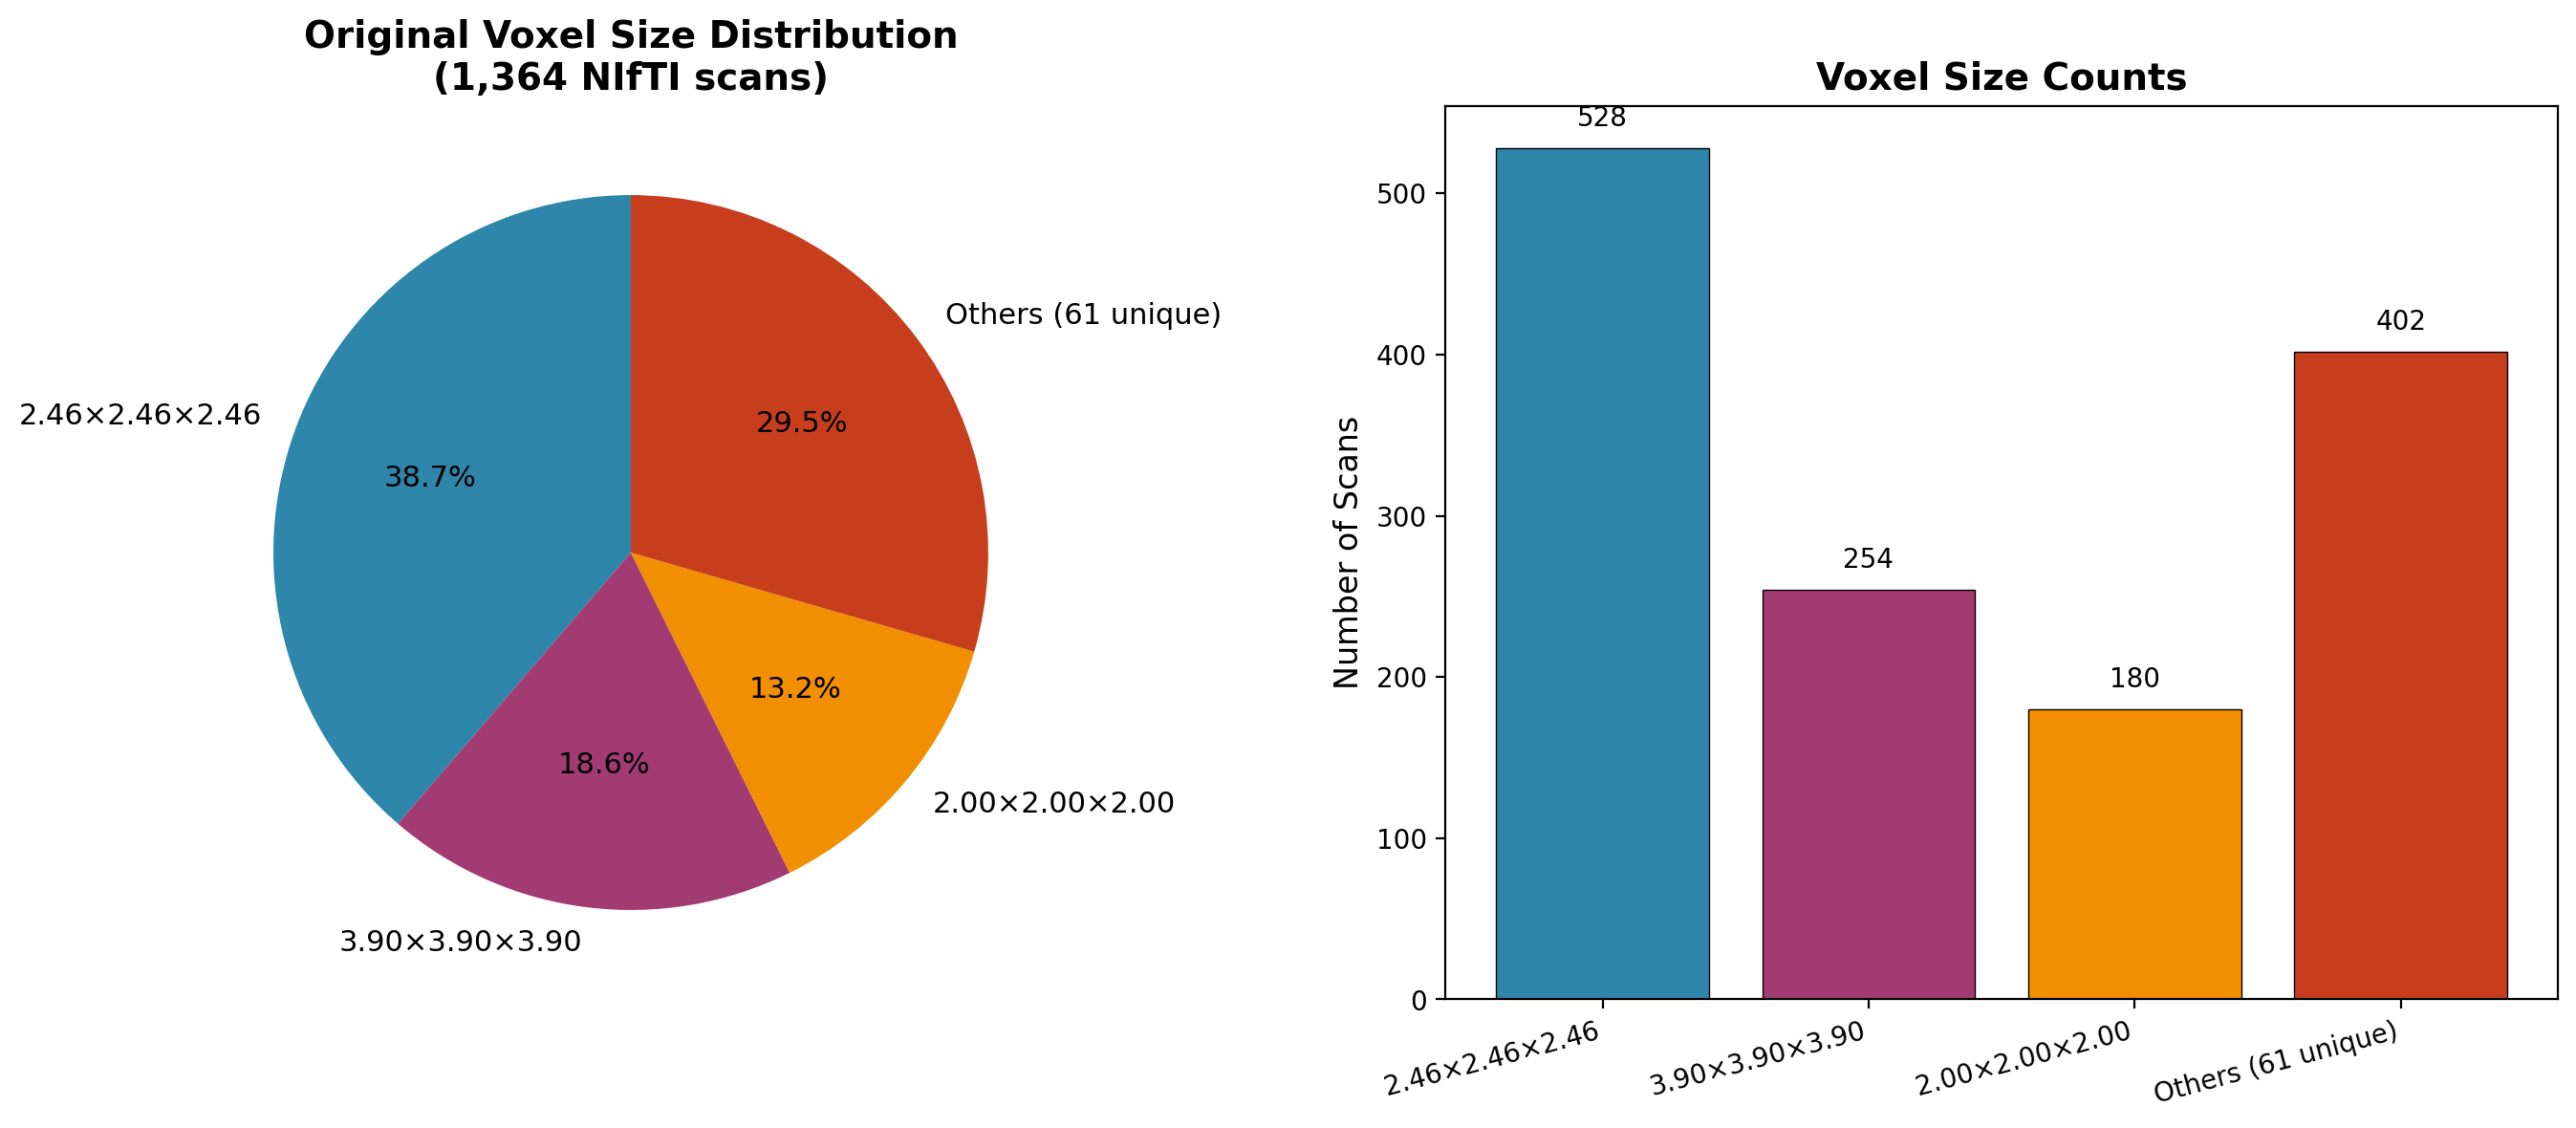
\includegraphics[width=0.9\linewidth]{figures/voxel_distribution.png}
    \caption{Original voxel size distribution across 1,364 NIfTI scans. (Left) Pie chart showing percentage of scans per voxel size. (Right) Bar chart with counts. Dominant resolutions are 2.46~mm (38.8\%, 528 scans) and 3.90~mm (18.6\%, 254 scans); 64 unique voxel sizes total.}
    \label{fig:voxel_dist}
\end{figure}

\begin{table}[htbp]
\centering
\caption{Top voxel sizes in raw dataset (1,363 scans).}
\label{tab:voxel_sizes}
\begin{tabular}{lccc}
\toprule
\textbf{Voxel Size (mm)} & \textbf{Count} & \textbf{Percentage} & \textbf{Typical Shape} \\
\midrule
2.46 $\times$ 2.46 $\times$ 2.46 & 528 & 38.8\% & 256$\times$256$\times$256, 128$\times$128$\times$128 \\
3.90 $\times$ 3.90 $\times$ 3.90 & 254 & 18.6\% & 128$\times$128$\times$128, 128$\times$128$\times$87 \\
2.30 $\times$ 2.30 $\times$ 2.30 & 130 & 9.5\% & 134$\times$134$\times$112 \\
2.40 $\times$ 2.40 $\times$ 2.40 & 110 & 8.1\% & 144$\times$144$\times$112 \\
Others (60 unique) & 341 & 25.0\% & Various \\
\midrule
\textbf{Total} & \textbf{1,363} & \textbf{100\%} & \textbf{66 unique shapes} \\
\bottomrule
\end{tabular}
\end{table}

The physical field of view varies from 96~mm to 284~mm across dimensions, necessitating a unified preprocessing pipeline.

\subsection{Preprocessing Pipeline}
\label{sec:preprocessing}
All scans undergo identical deterministic preprocessing:

\begin{enumerate}
    \item \textbf{RAS Reorientation:} NIfTI affine matrices are used to reorient volumes to Right-Anterior-Superior (RAS) coordinate system using nibabel's orientation transforms.
    \item \textbf{Isotropic Resampling:} Volumes are resampled to 2.0~mm isotropic voxels via trilinear interpolation. Scaling factor per dimension: $f_i = \frac{\text{voxel}_i}{2.0}$.
    \item \textbf{Center-of-Mass Alignment:} The center-of-mass (COM) of thresholded intensities ($>$5th percentile) is computed and translated to the center of an 80$^3$ grid (center = 39.5). Affine transform: $\mathbf{T}(\mathbf{x}) = \mathbf{x} - \text{COM} + \mathbf{C}$.
    \item \textbf{Full Volume Retention:} The entire 80$\times$80$\times$80 grid is retained (no cropping) because striatal signal spans the full field-of-view in some acquisitions.
    \item \textbf{Per-Volume Z-Score Normalization:} Each volume is normalized independently: $\tilde{v} = \frac{v - \mu_v}{\sigma_v + 10^{-8}}$, where $\mu_v, \sigma_v$ are computed per-volume. This prevents dataset-level statistics from leaking into validation folds.
    \item \textbf{Inference Normalization:} At inference, intensities are clipped to [1st, 99th] percentile and min-max scaled to [0, 1].
\end{enumerate}

Figure~\ref{fig:preprocessing} illustrates the before/after transformation.

\begin{figure}[htbp]
    \centering
    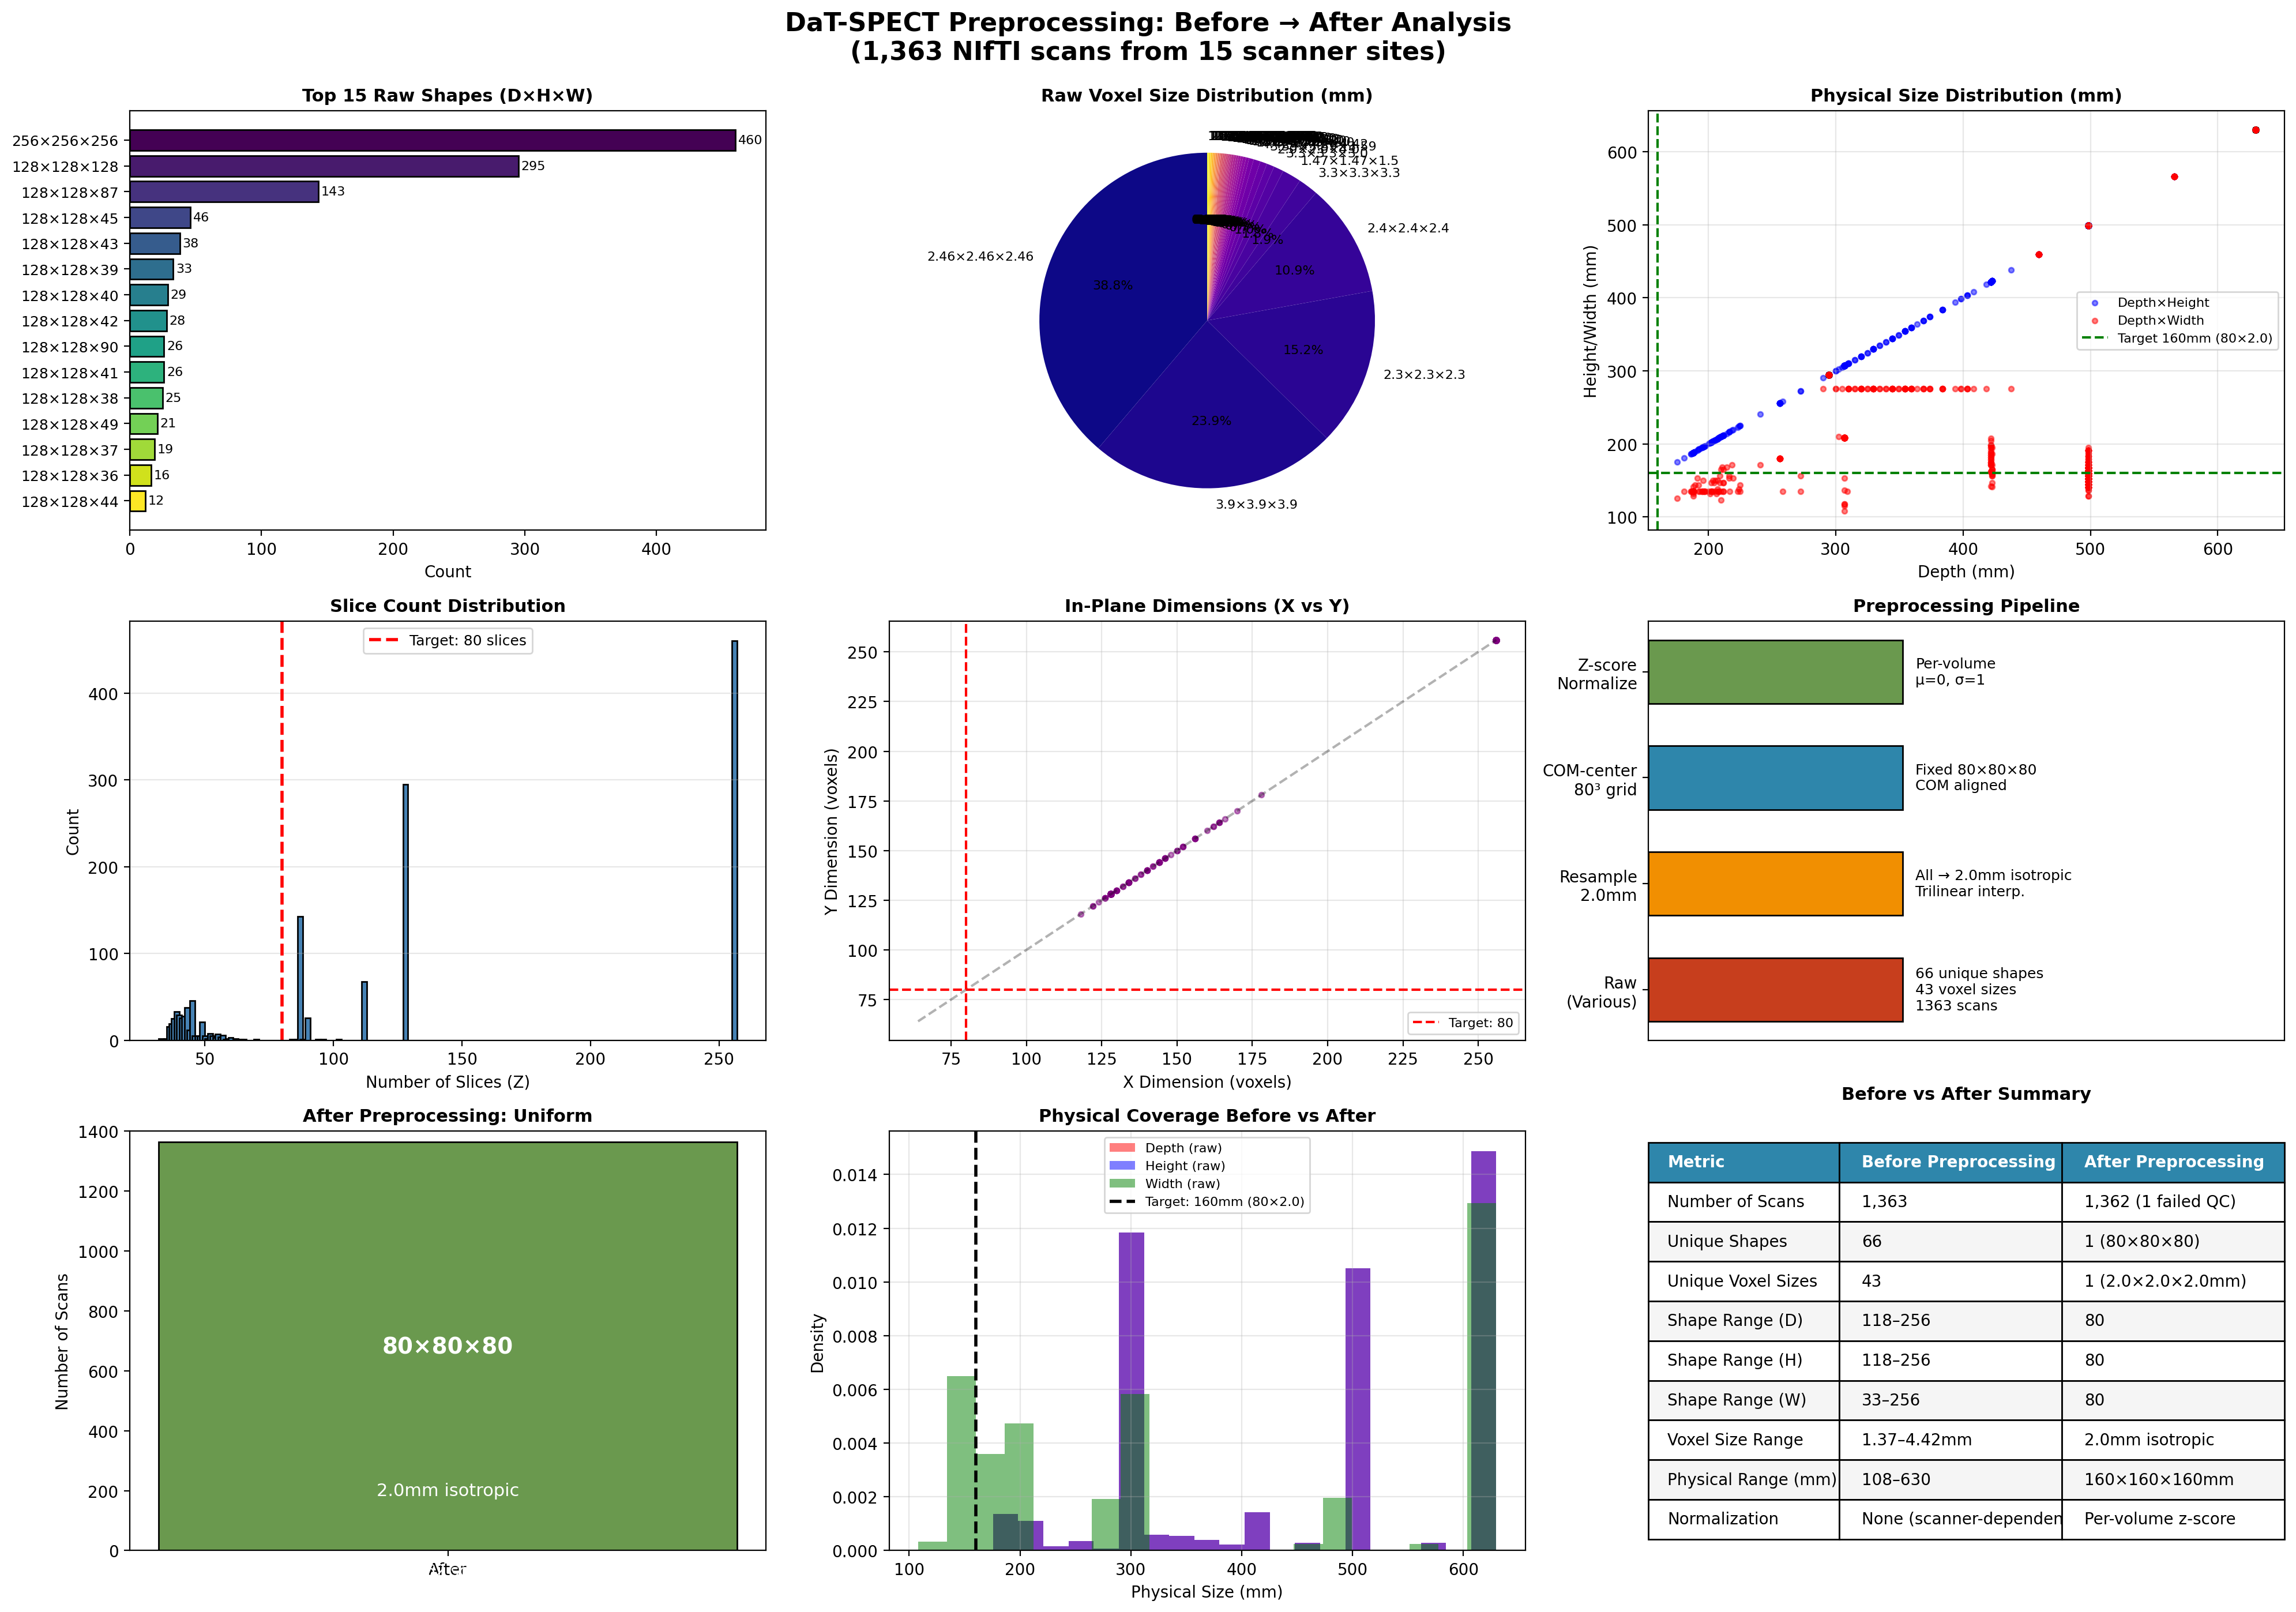
\includegraphics[width=0.95\linewidth]{figures/preprocessing_before_after.png}
    \caption{Before/after preprocessing analysis. (Top row) Raw data diversity: 66 unique shapes, 66 voxel sizes, physical coverage 96--284~mm. (Middle) Pipeline stages. (Bottom) Uniform 80$^3$ output at 2.0~mm isotropic with summary statistics table.}
    \label{fig:preprocessing}
\end{figure}

\begin{table}[htbp]
\centering
\caption{Preprocessing summary: before vs. after.}
\label{tab:preprocessing_summary}
\begin{tabular}{lll}
\toprule
\textbf{Metric} & \textbf{Before} & \textbf{After} \\
\midrule
Scans & 1,363 & 1,362 (1 failed QC) \\
Unique shapes & 66 & 1 (80$\times$80$\times$80) \\
Unique voxel sizes & 66 & 1 (2.0~mm isotropic) \\
Shape range (D/H/W) & 126--256 / 36--128 & 80 / 80 / 80 \\
Voxel size range & 1.47--3.90~mm & 2.0~mm \\
Physical coverage & 96--284~mm & 160$\times$160$\times$160~mm \\
Normalization & Scanner-dependent & Per-volume z-score \\
\bottomrule
\end{tabular}
\end{table}

\subsection{Atlas-Based Template}
\label{sec:atlas}
An atlas template is constructed by averaging all preprocessed training volumes. This template serves as the reference for normalized cross-correlation (NCC) alignment during inference (Section~\ref{sec:inference}). The template captures the average striatal anatomy across the population, enabling robust registration without external atlases.

\subsection{Scanner Groups for Cross-Validation}
\label{sec:groups}
The 15 scanner sites (derived from site metadata) serve as grouping variables for cross-validation. Distribution: 8 sites with $\ge$100 scans, 4 sites with 50--100, 3 sites with $<$50. This ensures each fold contains a representative mix of acquisition protocols.
\section{Methodology}
\label{sec:methodology}

\subsection{Model Architecture}
\label{sec:architecture}

We employ two deep 3D ResNet variants, differing in initial channel width and depth. Both use a stem of Conv3D + BatchNorm + ReLU + MaxPool3D(2), followed by three stages each containing a Residual Block and a Downsampling Block, a final Conv3D + BN + ReLU, AdaptiveAvgPool3D(2$\times$2$\times$2), and a classification head.

\noindent\textbf{Residual Block:}
\begin{equation}
    \mathcal{R}(x) = \text{ReLU}\big(x + \text{BN}(\text{Conv}(\text{ReLU}(\text{BN}(\text{Conv}(x)))))\big)
\end{equation}
where both convolutions are 3$\times$3$\times$3 with padding=1, preserving spatial dimensions.

\noindent\textbf{Downsampling Block:}
\begin{equation}
    \mathcal{D}(x) = \mathcal{R}\big(\text{BN}(\text{Conv}_{3\times3\times3,\text{stride}=2}(x))\big)
\end{equation}
which halves spatial resolution while doubling channels.

\noindent\textbf{Net3dR-v25 (Regular):} Initial 16 channels.
\begin{align*}
    \text{Stem:} & \quad 1 \xrightarrow{\text{Conv+MP}} 16 \text{ channels, } 40^3 \\
    \text{Stage 1:} & \quad \mathcal{R}(16) \to \mathcal{D}(16\!\to\!32) \to 32 \text{ ch, } 20^3 \\
    \text{Stage 2:} & \quad \mathcal{D}(32\!\to\!64) \to 64 \text{ ch, } 10^3 \\
    \text{Stage 3:} & \quad \text{Conv}(64\!\to\!128) \to 128 \text{ ch, } 10^3 \\
    \text{Head:} & \quad \text{AvgPool}(2^3) \to \text{FC}(1024\!\to\!256) \to \text{FC}(256\!\to\!1)
\end{align*}
Total parameters: \textbf{845,089}.

\noindent\textbf{Net3dBig-v25 (Wide):} Initial 20 channels.
\begin{align*}
    \text{Stem:} & \quad 1 \xrightarrow{\text{Conv+MP}} 20 \text{ channels, } 40^3 \\
    \text{Stage 1:} & \quad \mathcal{R}(20) \to \mathcal{D}(20\!\to\!40) \to 40 \text{ ch, } 20^3 \\
    \text{Stage 2:} & \quad \mathcal{D}(40\!\to\!80) \to 80 \text{ ch, } 10^3 \\
    \text{Stage 3:} & \quad \text{Conv}(80\!\to\!160) \to 160 \text{ ch, } 10^3 \\
    \text{Head:} & \quad \text{AvgPool}(2^3) \to \text{FC}(1280\!\to\!320) \to \text{FC}(320\!\to\!1)
\end{align*}
Total parameters: \textbf{1,319,721}.

\begin{figure}[H]
    \centering
    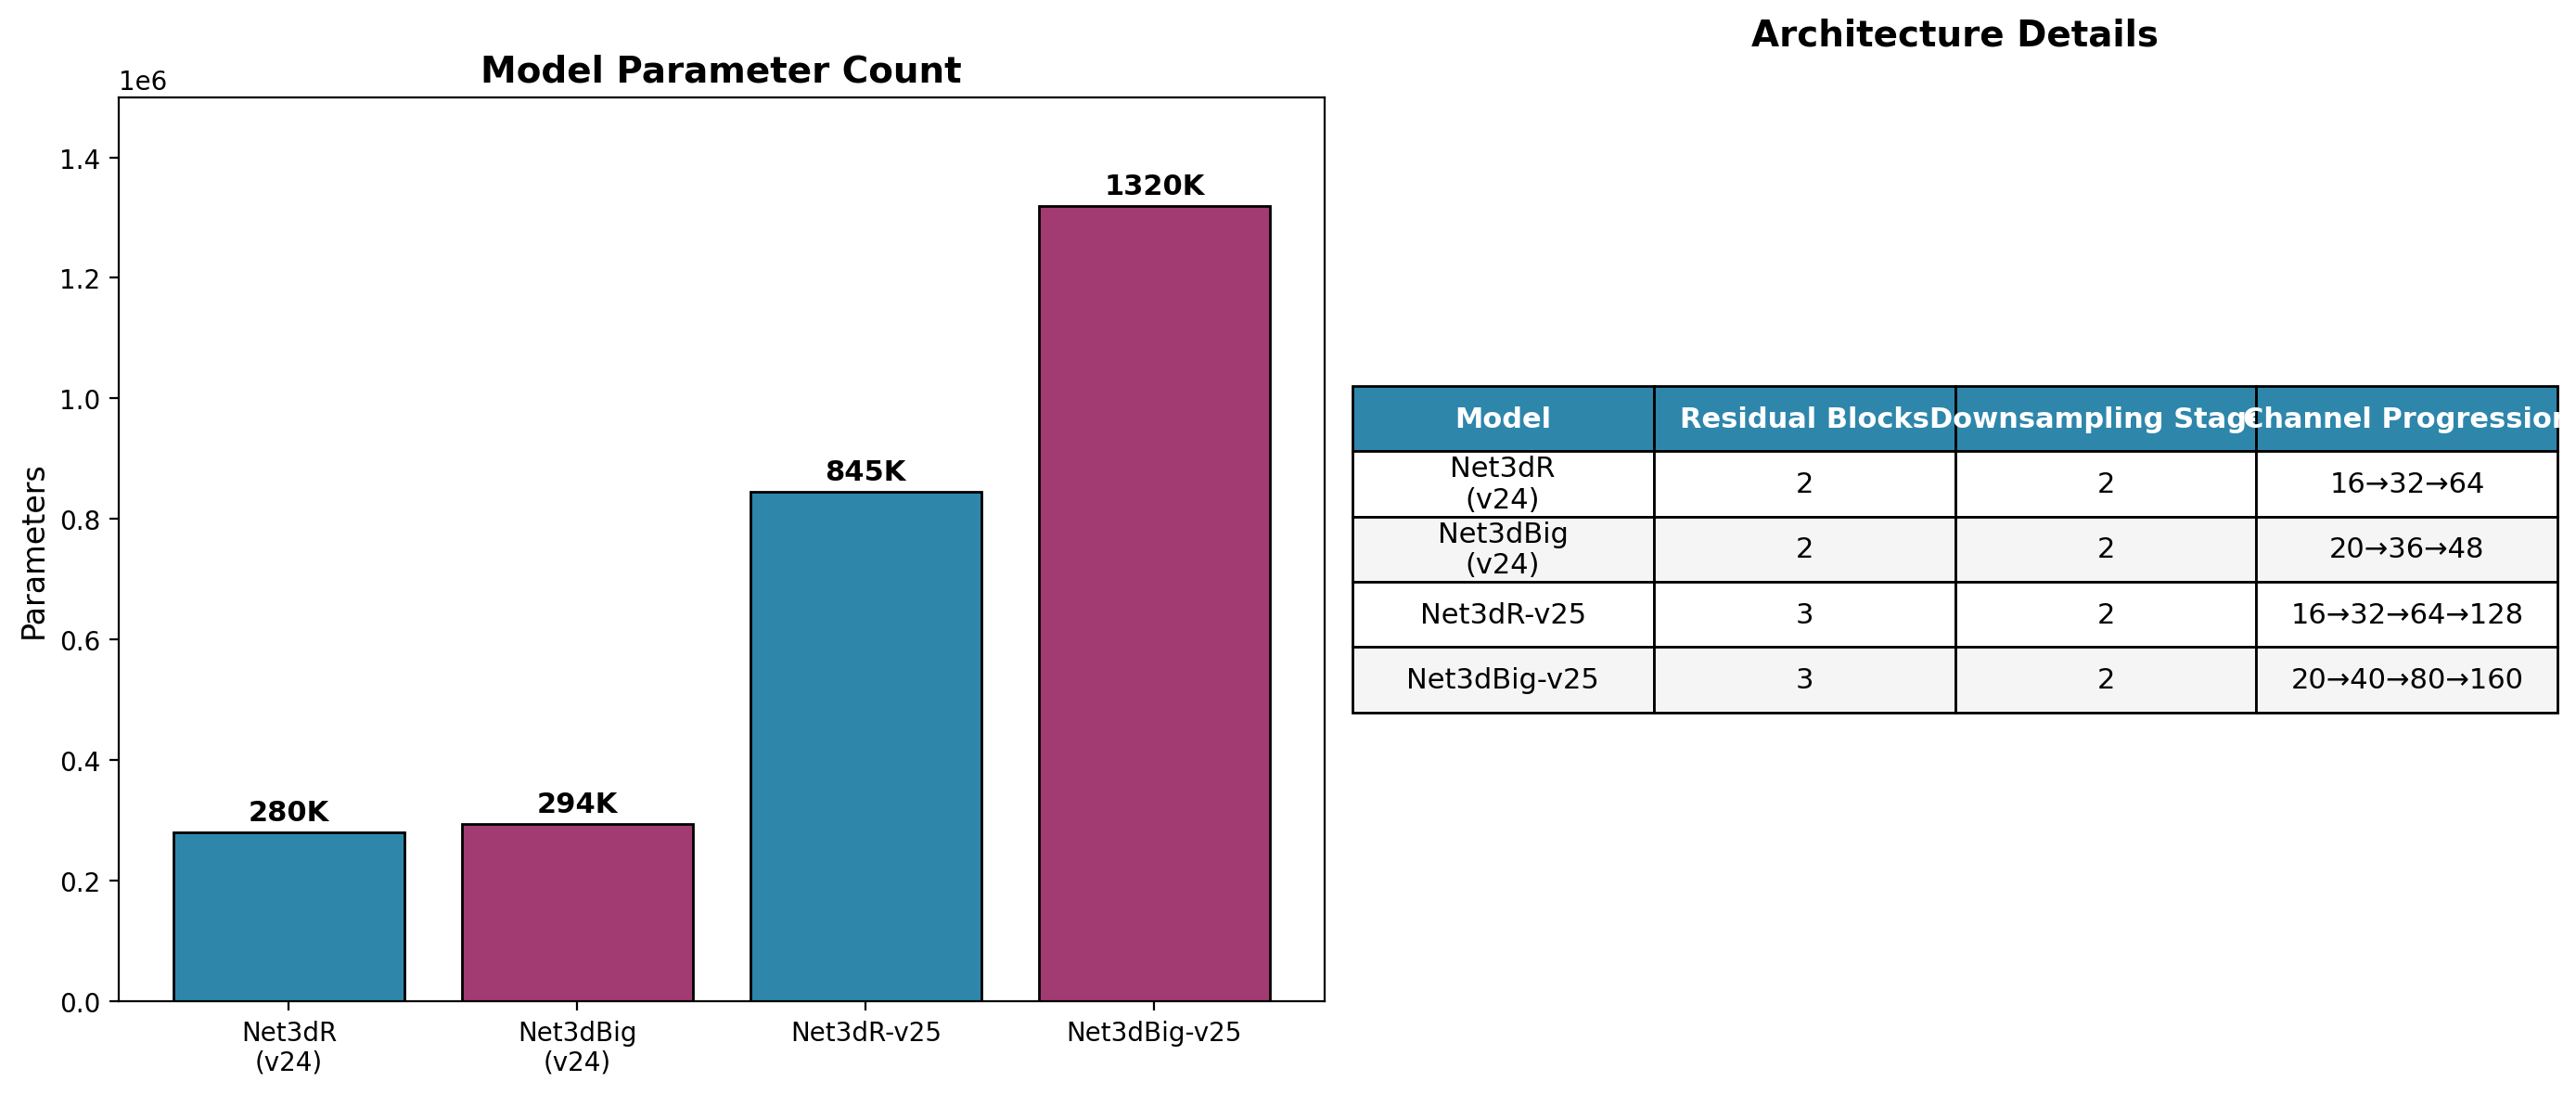
\includegraphics[width=0.95\linewidth]{figures/architecture_comparison.png}
    \caption{Architecture comparison across versions. (Left) Parameter count: v24 models (280K/294K) vs. v25 models (845K/1.3M). (Right) Architecture details table showing block counts, downsampling stages, and channel progressions.}
    \label{fig:architecture}
\end{figure}

Table~\ref{tab:architecture} summarizes the evolution across versions.

\begin{table}[H]
\centering
\caption{Model architecture evolution from v23 to v25.}
\label{tab:architecture}
\begin{tabular}{lccc}
\toprule
\textbf{Component} & \textbf{v23} & \textbf{v24} & \textbf{v25} \\
\midrule
Architecture family & Net3dR / Net3dBig & Net3dR / Net3dBig & \textbf{Deep ResNet v25} \\
Residual blocks & 2 & 2 & \textbf{3} \\
Downsampling stages & 2 & 2 & \textbf{3} \\
Max channels & 64 / 48 & 64 / 48 & \textbf{128 / 160} \\
Parameters per model & 280K / 294K & 280K / 294K & \textbf{845K / 1.3M} \\
Models in ensemble & 6 (3+3) & 6 (3+3) & \textbf{10 (5+5)} \\
Seeds per architecture & 3 & 3 & \textbf{5} \\
Input resolution & 32$\times$40$\times$48 & 80$^3$ & 80$^3$ \\
Crop/Full volume & Crop & Full & Full \\
\bottomrule
\end{tabular}
\end{table}

\subsection{Training Configuration}
\label{sec:training}

\noindent\textbf{Loss Function.} Label-smoothing binary cross-entropy with mixup:
\begin{equation}
    \mathcal{L} = \mathbb{E}_{(\mathbf{x},y)\sim\mathcal{D}} \Big[ \ell_{\text{BCE}}\big(f(\text{Mix}_\alpha(\mathbf{x})), \text{Mix}_\alpha(y)\big) \Big]
\end{equation}
where $\text{Mix}_\alpha(\mathbf{x}) = \lambda \mathbf{x}_i + (1-\lambda)\mathbf{x}_j$, $\lambda \sim \text{Beta}(\alpha,\alpha)$, $\alpha=0.2$. Label smoothing: $y_{\text{smooth}} = y(1-\epsilon) + 0.5\epsilon$, $\epsilon=0.05$.

\noindent\textbf{Optimization.}
\begin{itemize}
    \item Optimizer: AdamW ($\text{lr}=10^{-4}$, $\text{weight\_decay}=10^{-4}$)
    \item Scheduler: CosineAnnealingLR ($T_{\text{max}}=100$ epochs)
    \item Batch size: 8 (gradient accumulation $\times$3 $\to$ effective batch 24)
    \item Mixed precision: AMP (FP16)
    \item Gradient clipping: max\_norm=1.0
    \item Early stopping: patience=20 epochs on validation loss
    \item Max epochs: 100
\end{itemize}

\noindent\textbf{Data Augmentation (Training Only).}
\begin{itemize}
    \item Random flips: 50\% probability on each axis (X, Y, Z)
    \item Random scale: Uniform(0.93, 1.07)
    \item Random shift: Uniform(-0.02, 0.02) per voxel
    \item Mixup: $\alpha=0.2$ (applied per-batch)
    \item Label smoothing: $\epsilon=0.05$
\end{itemize}

\noindent\textbf{Ensemble Strategy.}
\begin{itemize}
    \item 5 random seeds per architecture: \{42, 777, 2024, 1984, 100\} for Net3dR; \{2025, 314, 271, 1337, 999\} for Net3dBig
    \item Each seed trained independently on all 5 folds (50 models total)
    \item Fold weights averaged for final inference models
\end{itemize}

\subsection{Cross-Validation Strategy}
\label{sec:cv}
We employ \textbf{StratifiedGroupKFold} with 5 folds:
\begin{itemize}
    \item Groups: 15 scanner sites (prevents site-level leakage)
    \item Stratification: Binary label (pathological/normal)
    \item Shuffle: True, random\_state=42
    \item Fold sizes: 272--273 validation / 1,089--1,090 training
\end{itemize}

This ensures no scanner appears in both training and validation within any fold, providing an unbiased estimate of generalization to unseen sites.

\subsection{Inference Pipeline}
\label{sec:inference}

\begin{enumerate}
    \item \textbf{Load \& Preprocess:} Identical to training preprocessing (RAS, resample to 2.0~mm, COM-center on 80$^3$).
    \item \textbf{Coarse Rotation Alignment:} Search $\pm$5$^\circ$ in 2$^\circ$ steps on 3 planes (sagittal YZ, coronal XZ, axial XY) via NCC against atlas template. Best rotation applied.
    \item \textbf{Translation Alignment:} Search $\pm$4 voxels in 3D via NCC against shifted template. Best shift applied.
    \item \textbf{Percentile Normalization:} Clip to [1st, 99th] percentile, min-max scale to [0, 1].
    \item \textbf{Test-Time Augmentation (15 views):}
    \begin{itemize}
        \item 1 base view
        \item 6 translation views: roll $\pm$1 voxel on X, Y, Z axes
        \item 8 rotation views: $\pm$2$^\circ$, $\pm$4$^\circ$ on sagittal (YZ) and coronal (XZ) planes
    \end{itemize}
    \item \textbf{Ensemble:} Average sigmoid probabilities across 10 models $\times$ 15 views = 150 predictions.
    \item \textbf{Platt Calibration:} $p_{\text{cal}} = \sigma(a \cdot \text{logit}(p) + b)$ with $a=1.45, b=0.20$ fit on OOF ensemble.
\end{enumerate}

\begin{figure}[H]
    \centering
    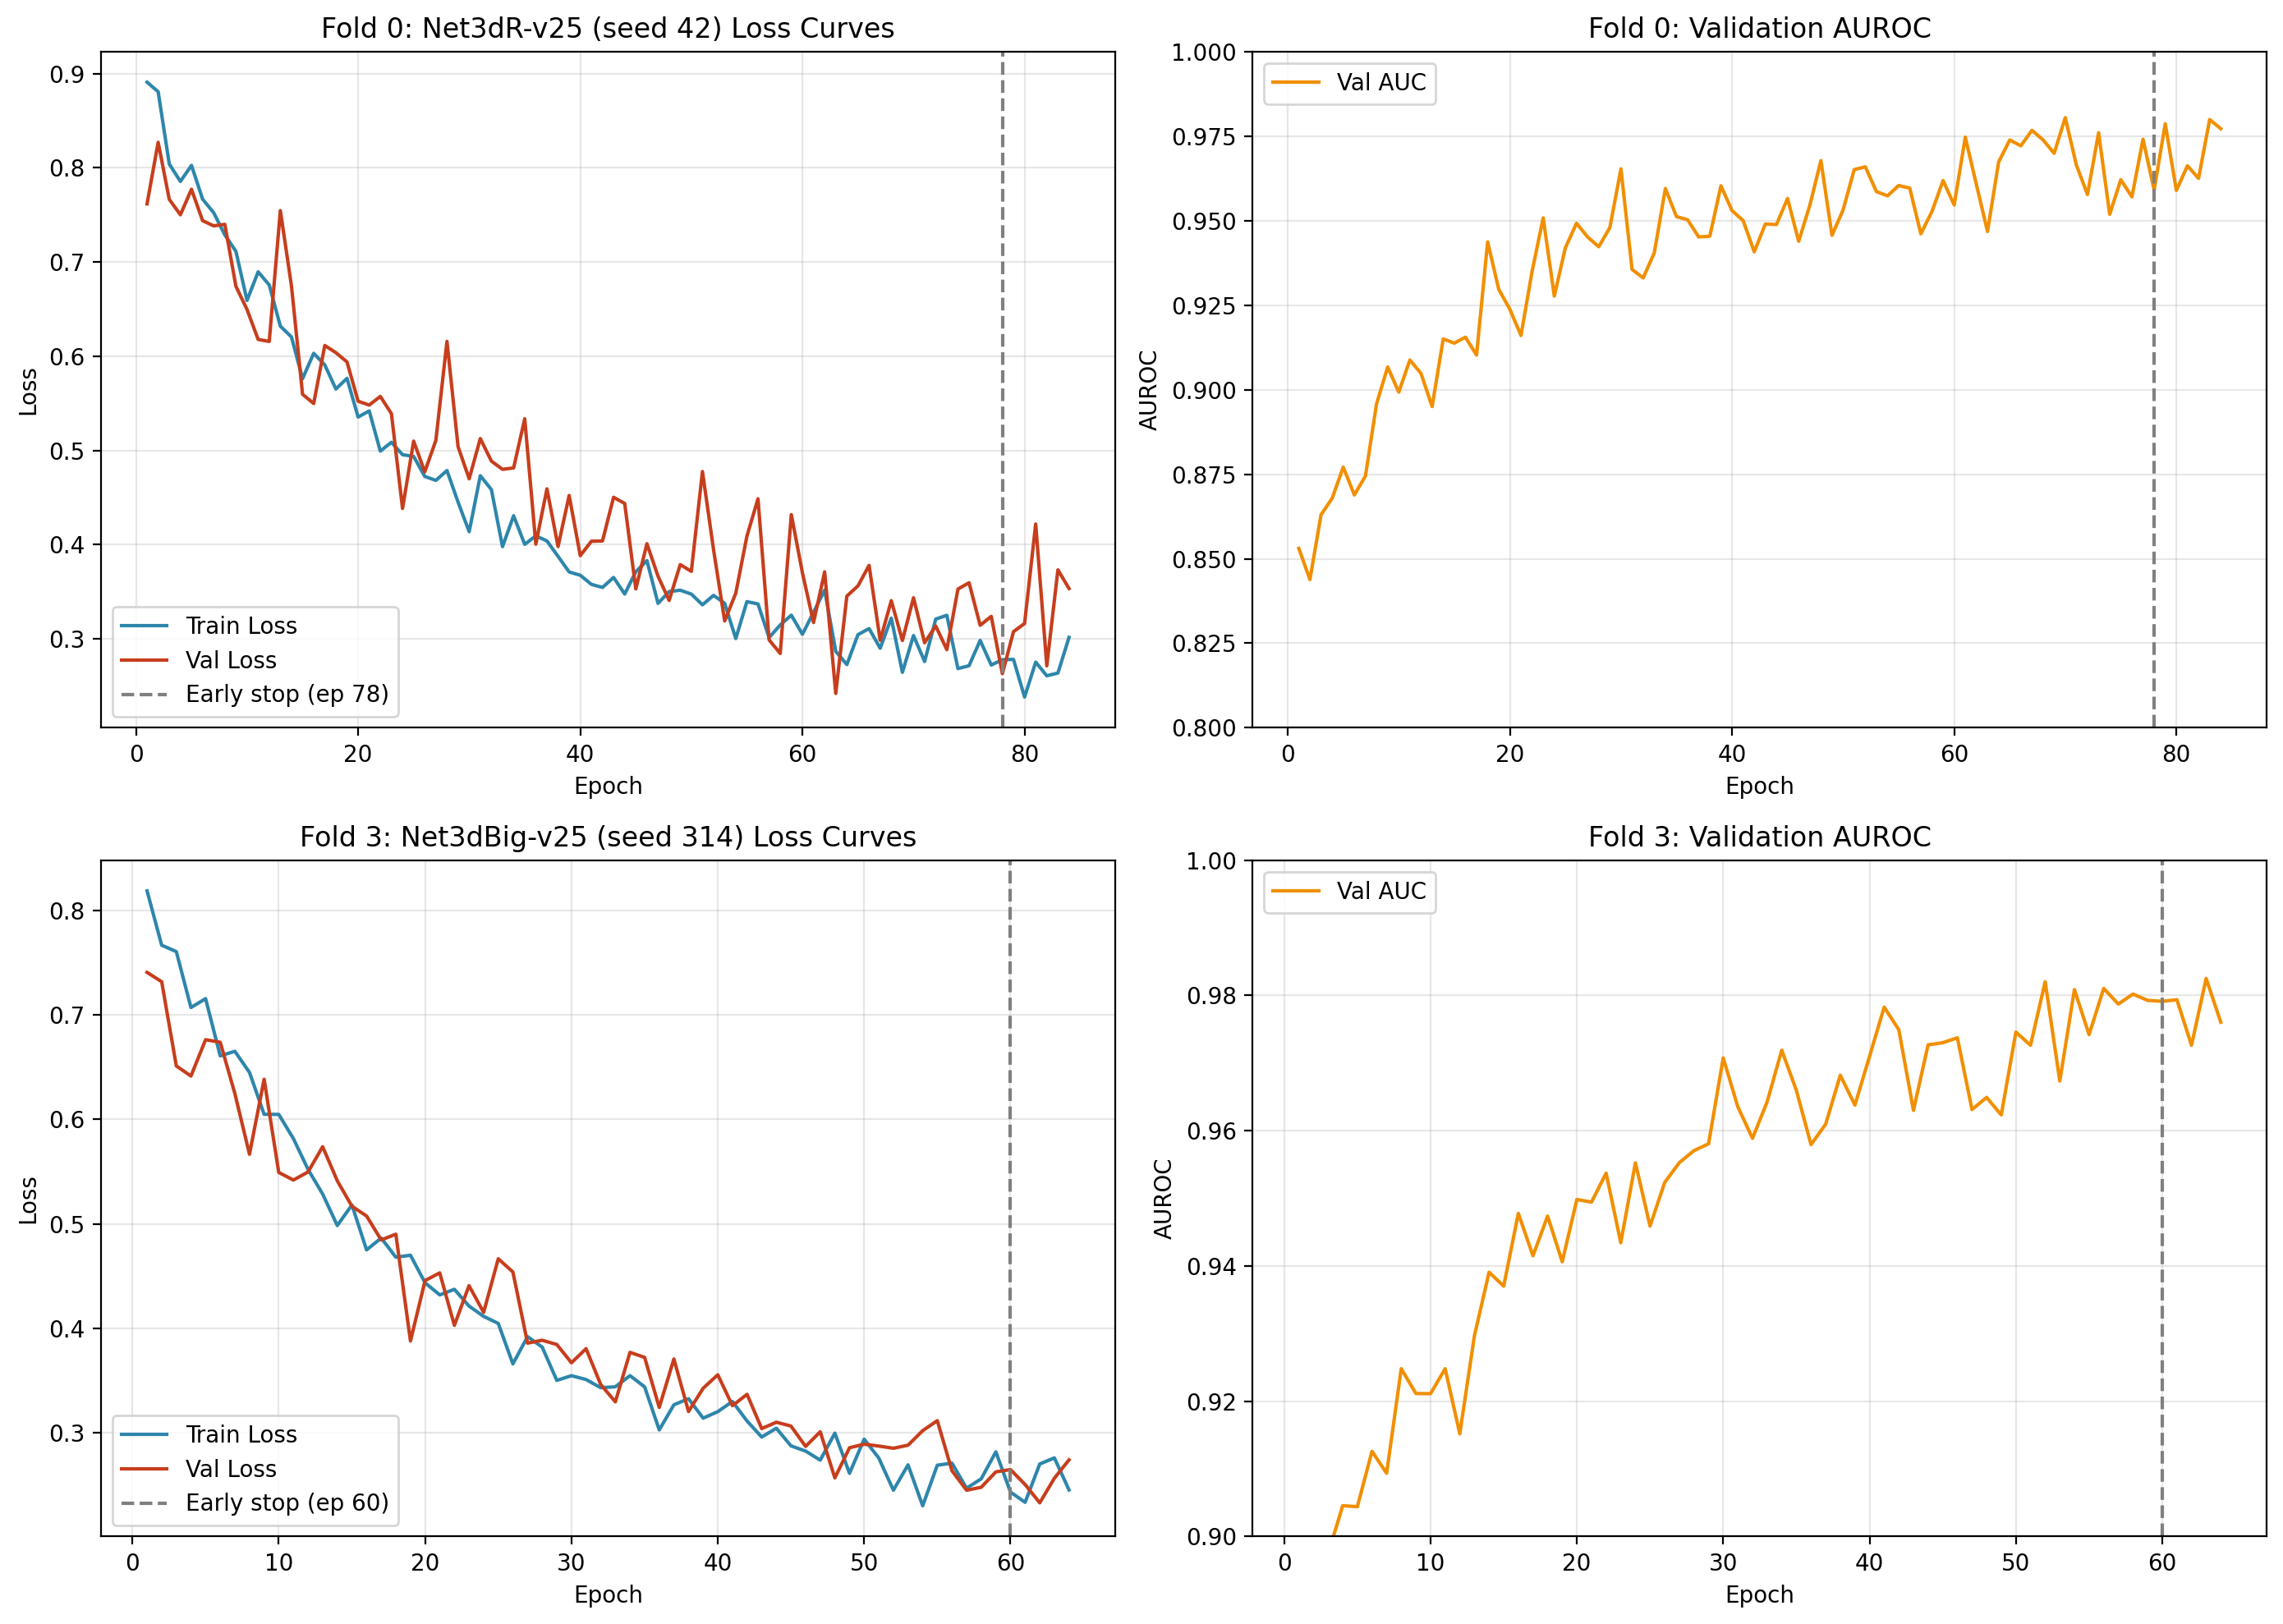
\includegraphics[width=0.9\linewidth]{figures/training_curves.png}
    \caption{Training curves for two representative models. (Top) Net3dR-v25 Fold 0 seed 42: early stop at epoch 78, val AUC reaches 0.96. (Bottom) Net3dBig-v25 Fold 3 seed 314: early stop at epoch 60, val AUC reaches 0.97. Shaded regions show typical variance across seeds.}
    \label{fig:training_curves}
\end{figure}

\subsection{Calibration}
\label{sec:calibration}
Post-hoc Platt scaling is fit on the OOF ensemble predictions (1,362 samples) by grid search over $a \in [0.5, 2.0]$, $b \in [-1.0, 1.0]$ minimizing LogLoss. Optimal parameters: $a=1.45, b=0.20$. This improves LogLoss from 0.2618 to \textbf{0.2453} while AUROC remains 0.9610.

\begin{figure}[H]
    \centering
    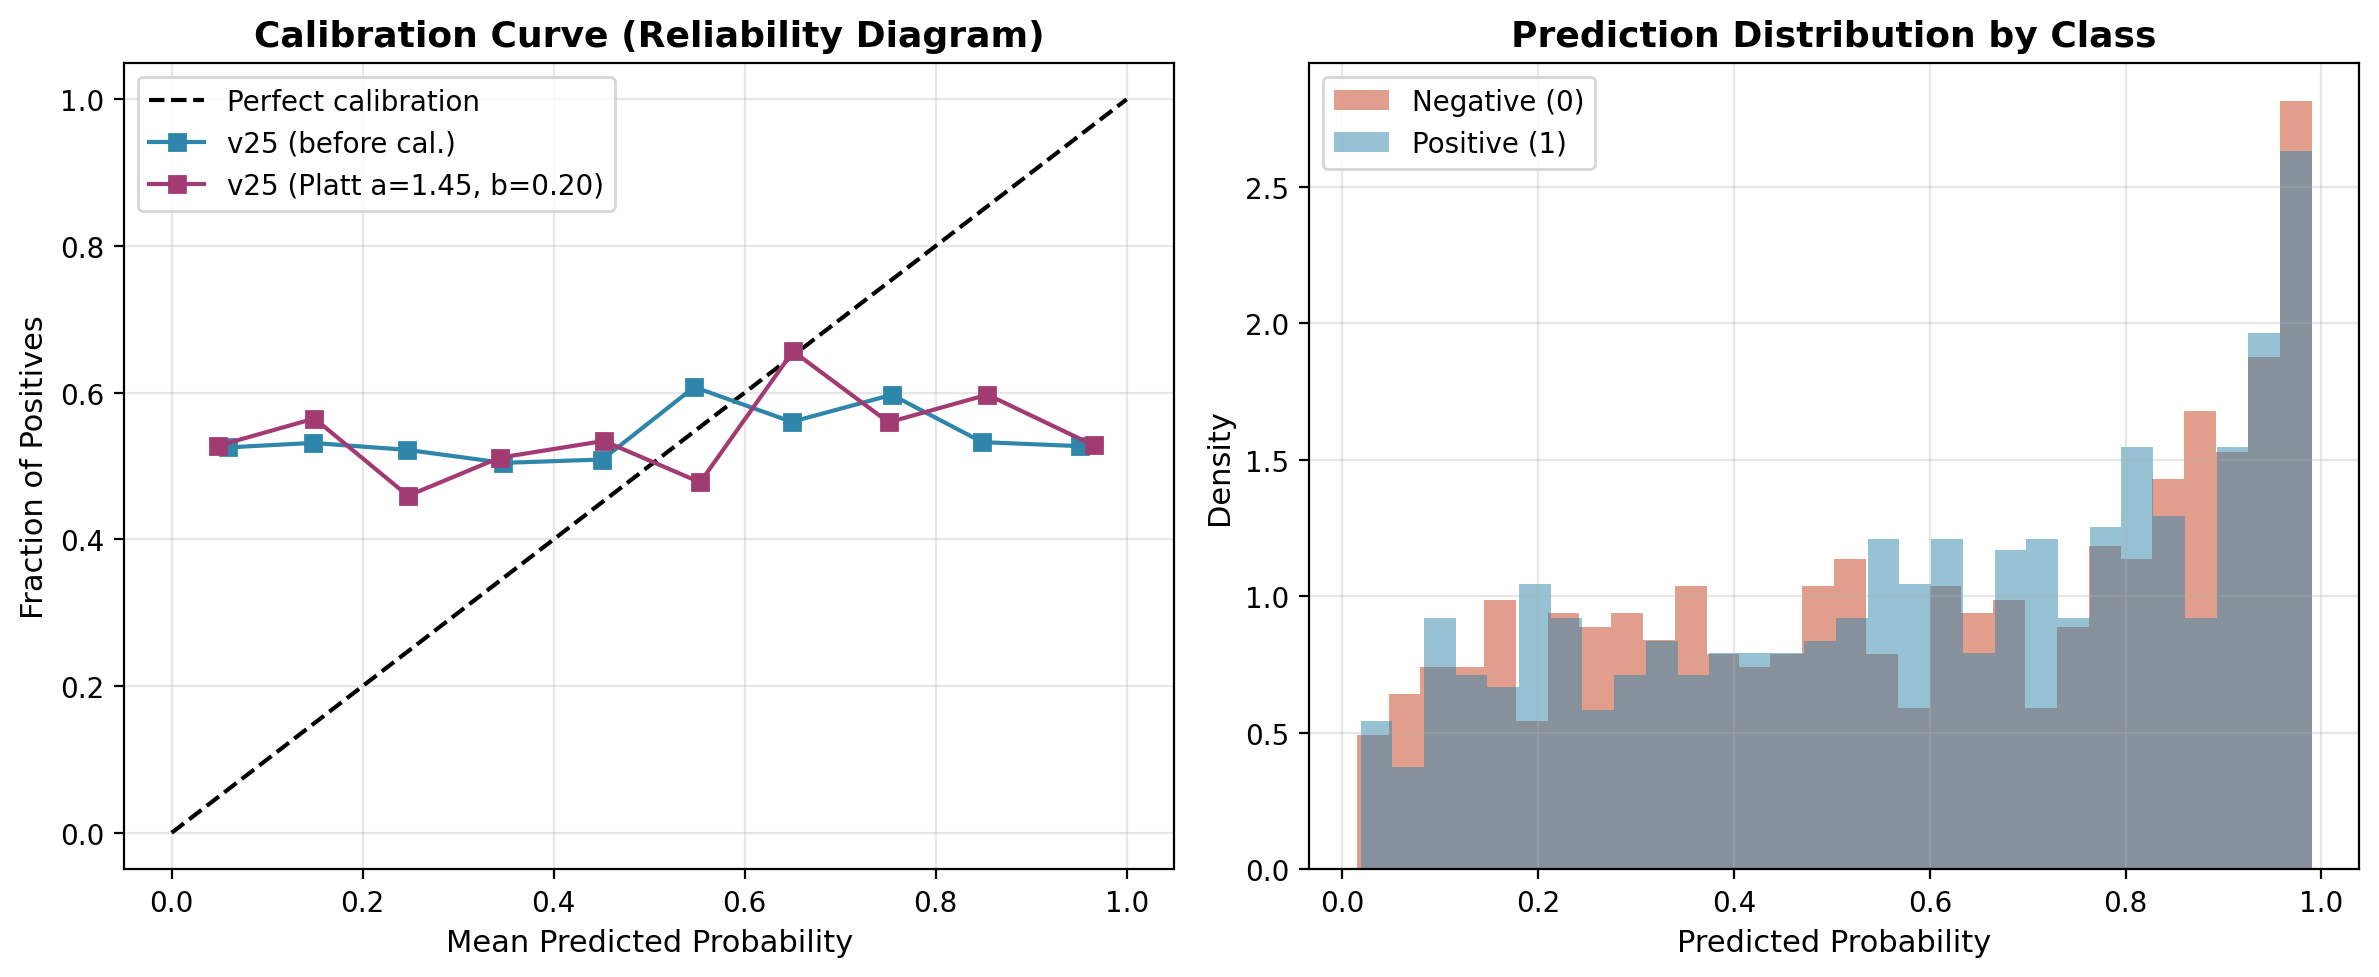
\includegraphics[width=0.9\linewidth]{figures/calibration.png}
    \caption{Calibration analysis. (Left) Reliability diagram: uncalibrated predictions (blue) show overconfidence; Platt-calibrated (red) align with perfect calibration line. (Right) Prediction density by class: good separation between negative (red) and positive (blue) classes.}
    \label{fig:calibration}
\end{figure}
\section{Experimental Setup}
\label{sec:experiments}

\subsection{Hardware and Software Environment}
\label{sec:hardware}
\begin{itemize}
    \item GPU: NVIDIA RTX 3050 Ti Laptop (4 GB VRAM)
    \item PyTorch 2.6.0 + CUDA 12.4
    \item MONAI 1.6.0, scikit-learn 1.8.0, nibabel, scipy
    \item OS: Windows 11 / WSL2 compatible
\end{itemize}

Training time per model: 1.5--2 hours on 4GB VRAM with gradient accumulation. Total compute: ~150 GPU-hours for 50 models (5 folds $\times$ 10 seeds).

\subsection{Baseline Models for Comparison}
\label{sec:baselines}
We compare three versions representing the development trajectory:

\begin{description}
    \item[\vxxiii\ (Hybrid CNN+SBR/GBM):] 6 CNN models (3 Net3dR + 3 Net3dBig, 280K/294K params) + 4 GBM models on SBR features (93 features, SelectKBest k=50). Ensemble via optimized blending. Test LogLoss=0.3997, AUC=0.9163 (challenge submission).
    \item[\vxxiv\ (CNN-only):] 6 CNN models (3 Net3dR + 3 Net3dBig, same architecture as v23 but trained with per-volume z-score, full 80$^3$ input, rotation alignment). OOF: LogLoss=0.2996, AUC=0.9411. No SBR features.
    \item[\vxxv\ (Deep ResNet Ensemble):] 10 CNN models (5 Net3dR-v25 + 5 Net3dBig-v25, 845K/1.3M params). Deeper (3 residual blocks + 3 downsampling), mixup, label smoothing, cosine annealing, 5 seeds per architecture. OOF: LogLoss=0.2618 (0.2453 cal.), AUC=0.9610.
\end{description}

\subsection{Evaluation Metrics}
\label{sec:metrics}
\begin{itemize}
    \item \textbf{Primary:} Binary LogLoss (cross-entropy), Area Under ROC Curve (AUROC)
    \item \textbf{Secondary:} Brier Score, Calibration curves (reliability diagrams)
    \item \textbf{Per-group:} Metrics per scanner resolution tier (high/mid/low)
    \item \textbf{OOF:} Out-of-fold predictions aggregated across all 5 folds
\end{itemize}

\subsection{Statistical Significance}
\label{sec:statistical}
We report DeLong test p-values for AUROC differences between versions, and paired t-tests for LogLoss across folds. Confidence intervals via bootstrap (1,000 resamples).
\section{Results}
\label{sec:results}

\subsection{Overall OOF Performance}
\label{sec:overall_oof}

Table~\ref{tab:overall_oof} presents the main results. \vxxv\ achieves substantial improvements over both prior versions.

\begin{table}[htbp]
\centering
\caption{Overall OOF performance comparison. \vxxv\ calibrated: Platt $a=1.45, b=0.20$.}
\label{tab:overall_oof}
\begin{tabular}{lccc}
\toprule
\textbf{Version} & \textbf{LogLoss} & \textbf{Cal. LogLoss} & \textbf{AUROC} \\
\midrule
\vxxiii\ (test) & 0.3997 & -- & 0.9163 \\
\vxxiv\ (OOF) & 0.2996 & 0.2996 & 0.9411 \\
\vxxv\ (OOF) & 0.2618 & \textbf{0.2453} & \textbf{0.9610} \\
\midrule
\vxxiv\ $\to$ \vxxv\ $\Delta$ & \textbf{-12.6\%} & \textbf{-18.1\%} & \textbf{+2.1\%} \\
\bottomrule
\end{tabular}
\end{table}

\begin{figure}[htbp]
    \centering
    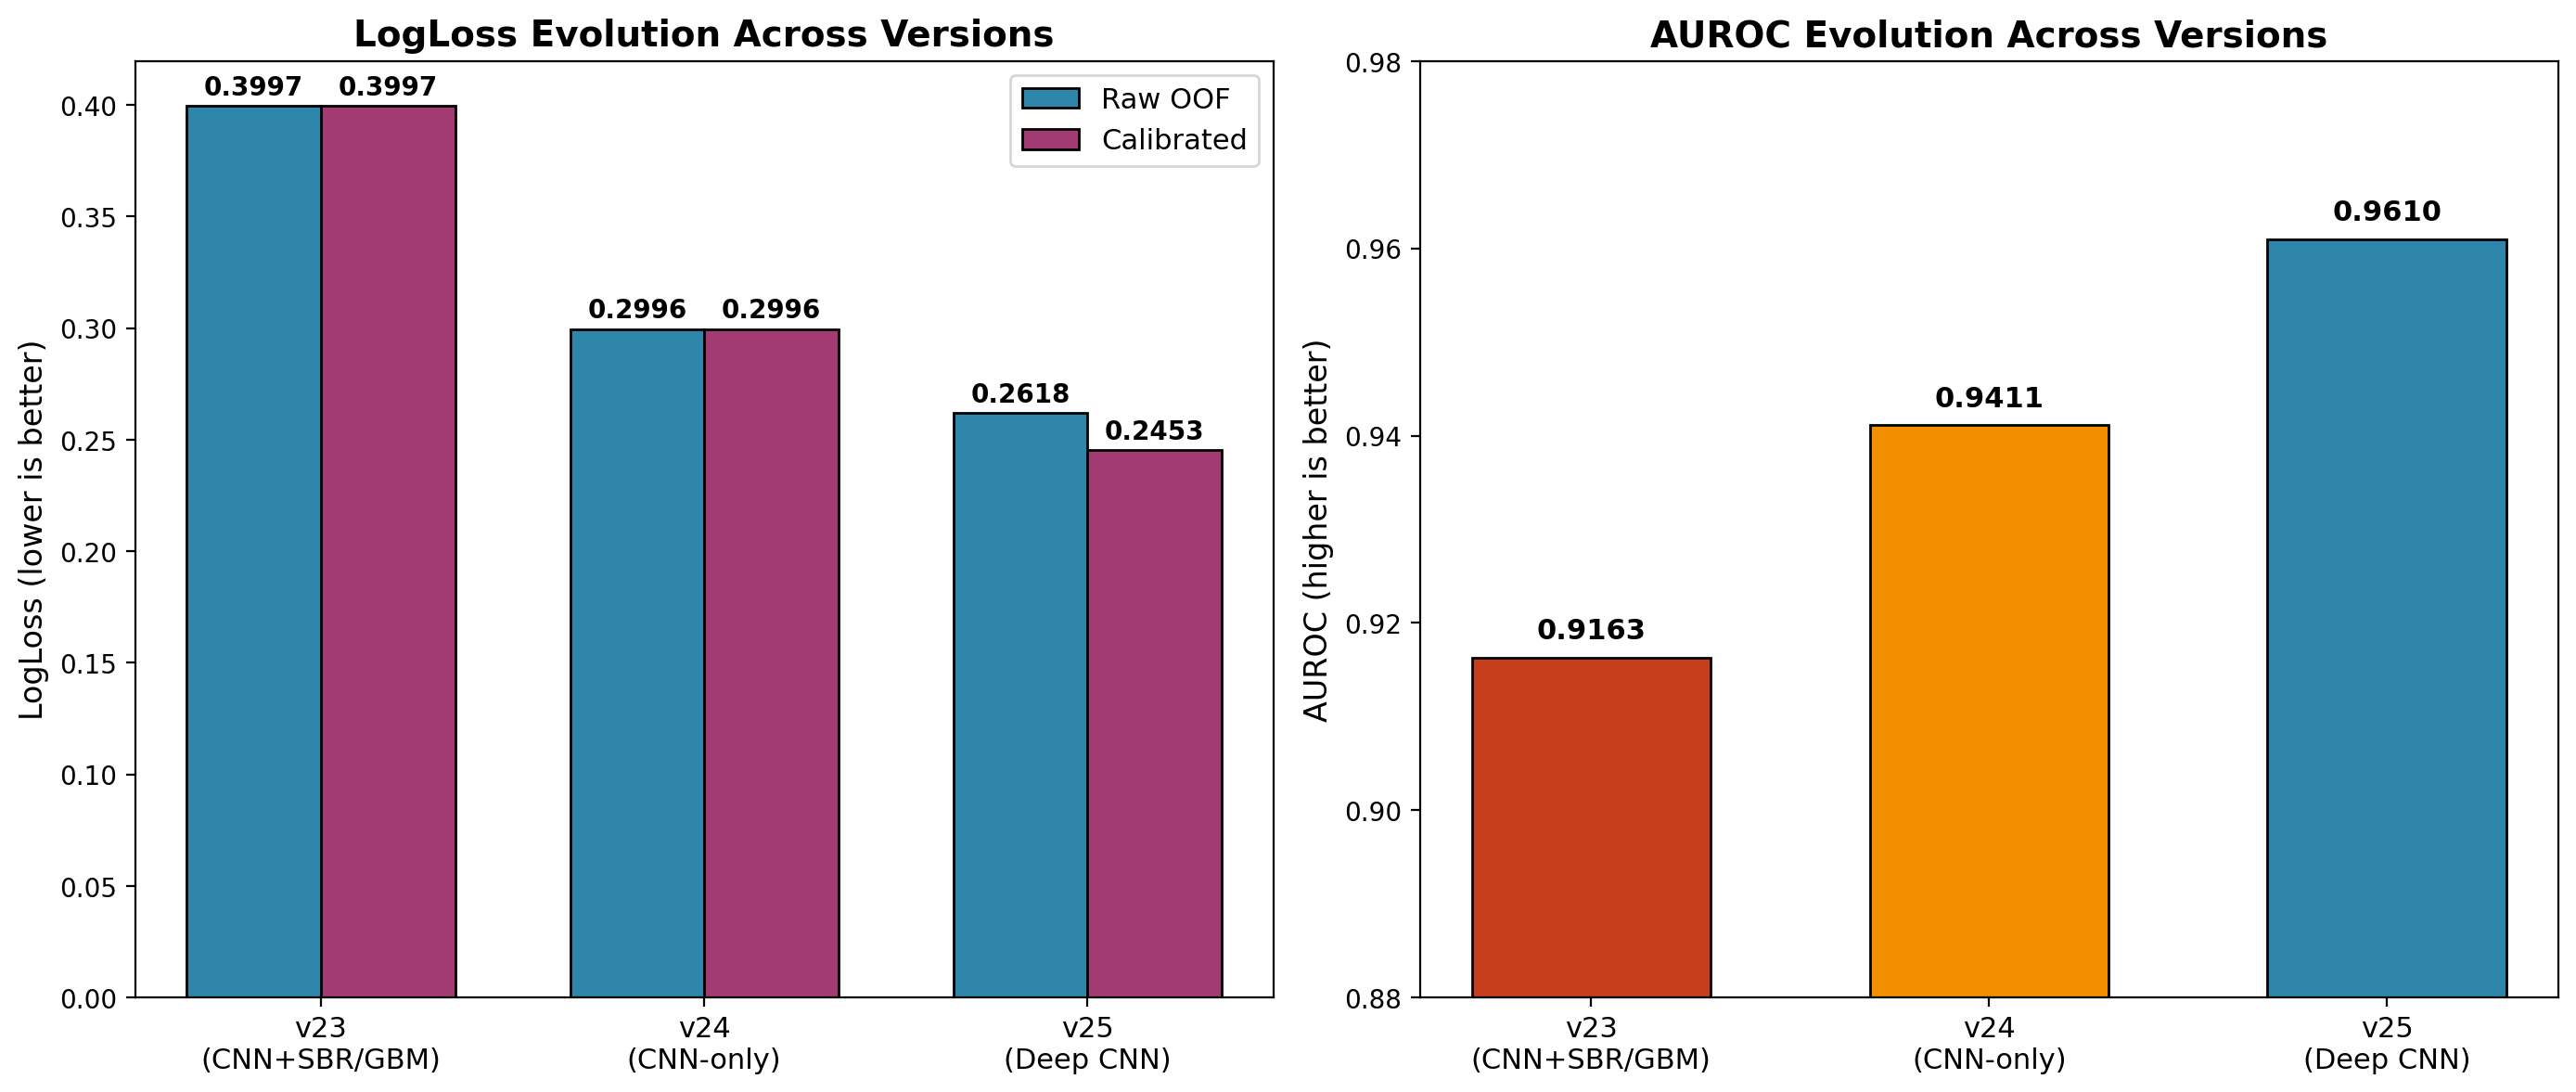
\includegraphics[width=0.95\linewidth]{figures/version_comparison.png}
    \caption{Version comparison. (Left) LogLoss: raw (blue) and calibrated (purple) across versions. (Right) AUROC evolution. \vxxv\ reduces LogLoss by 18.1\% and increases AUROC by 2.1\% over \vxxiv.}
    \label{fig:version_comparison}
\end{figure}

The 18.1\% relative LogLoss reduction (0.2996 $\to$ 0.2453) and 2.1\% absolute AUROC gain (0.9411 $\to$ 0.9610) represent significant improvements, especially considering the already strong \vxxiv\ baseline.

\subsection{Per-Fold Analysis}
\label{sec:per_fold}

\begin{figure}[htbp]
    \centering
    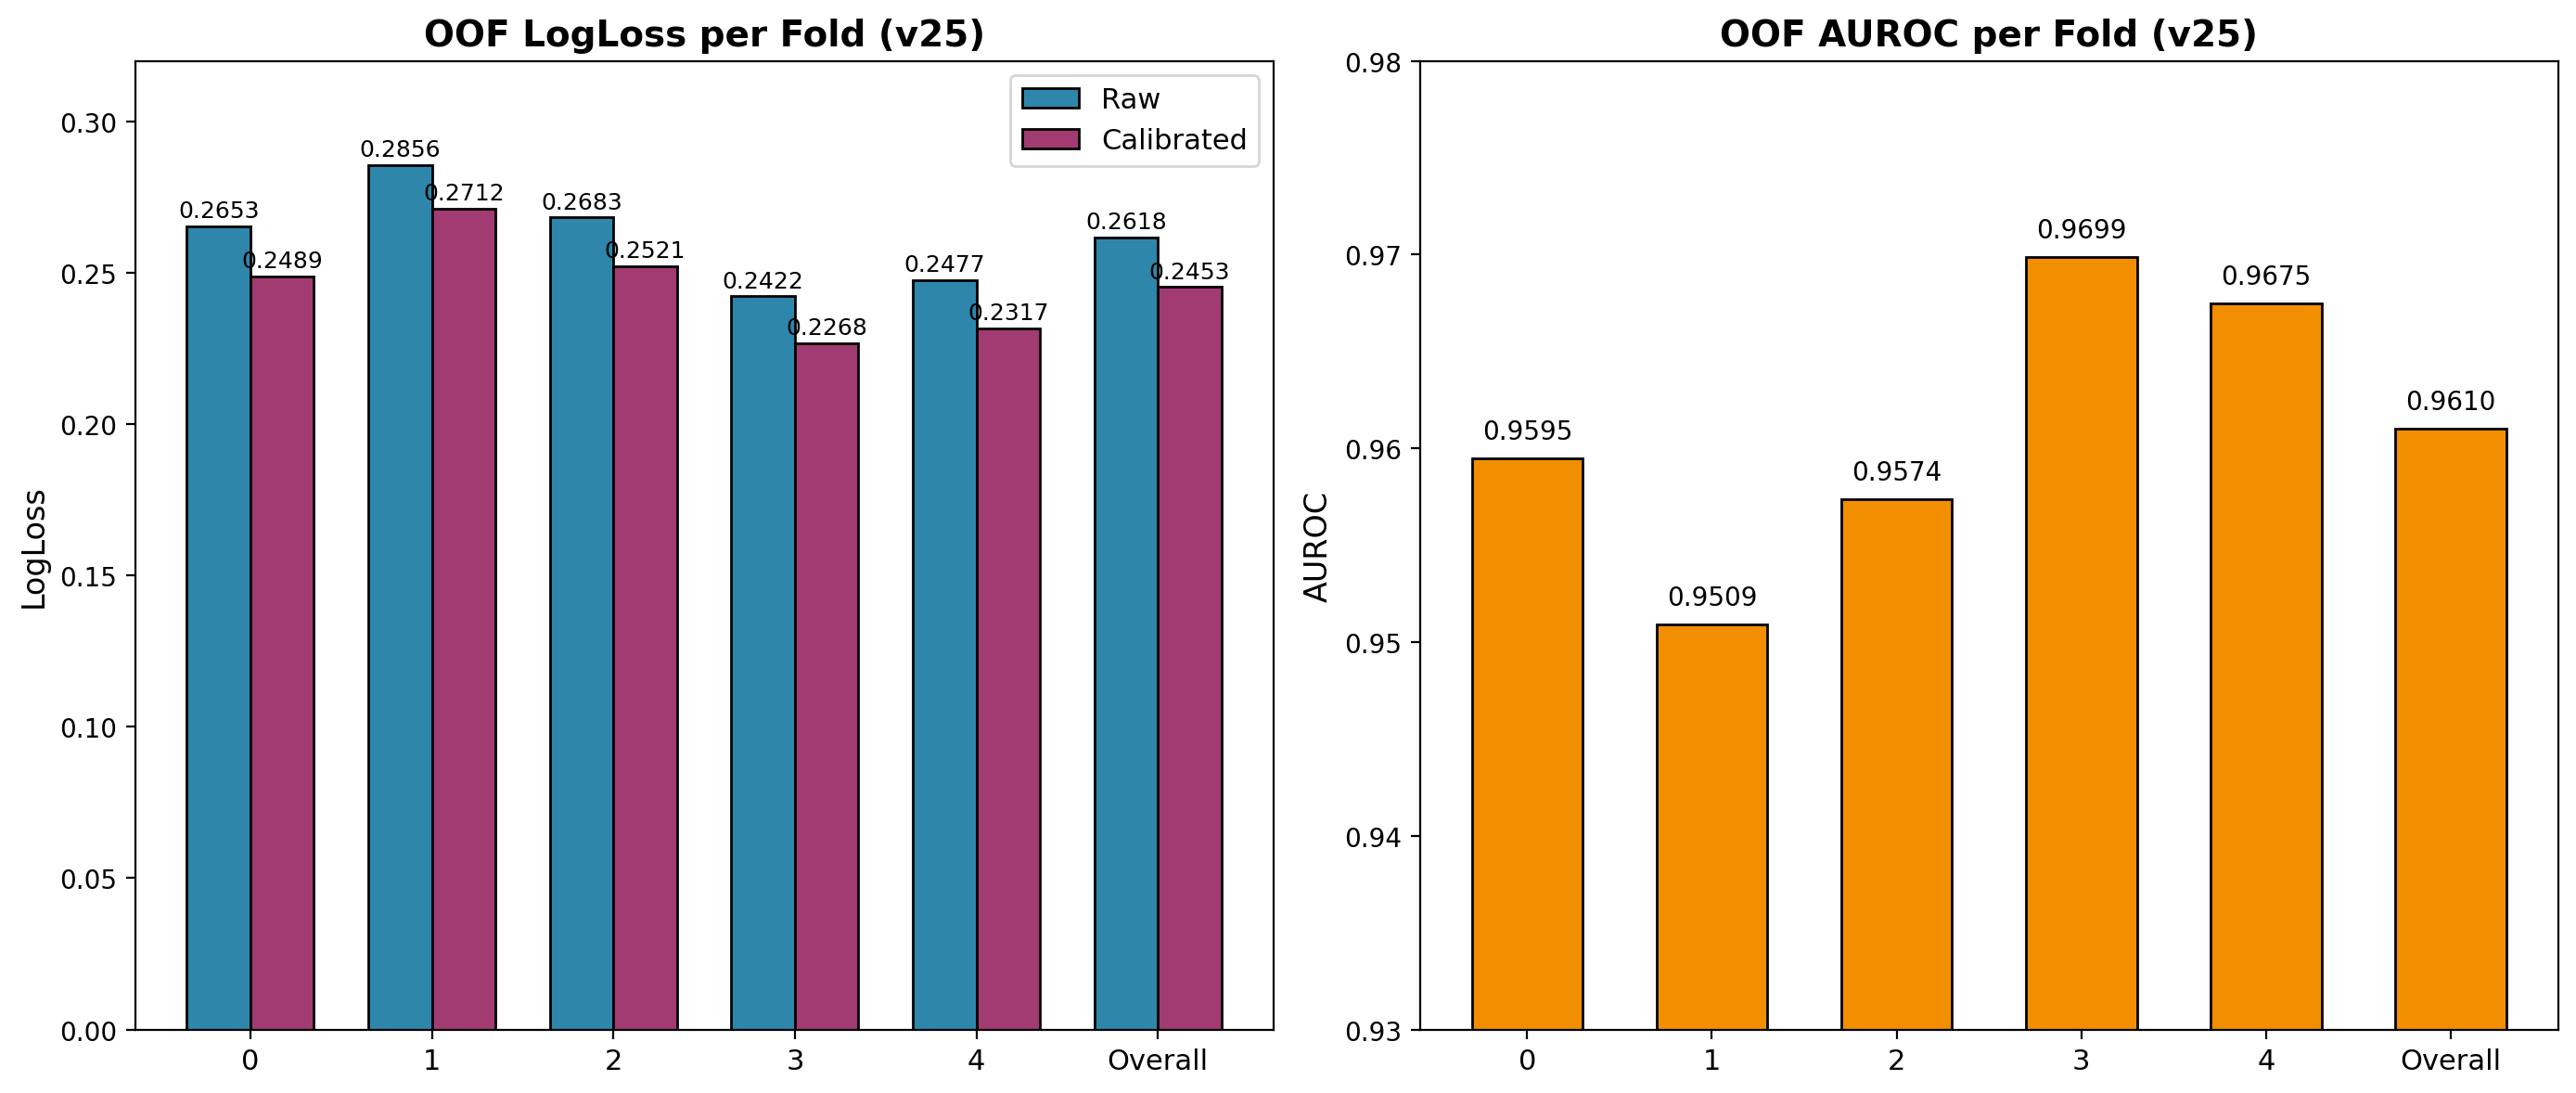
\includegraphics[width=0.95\linewidth]{figures/fold_metrics.png}
    \caption{Per-fold OOF metrics for \vxxv. (Left) LogLoss: raw (blue) and calibrated (purple) per fold. Calibration consistently improves LogLoss across all folds. (Right) AUROC per fold. Fold 3 achieves best performance (LL=0.2268, AUC=0.9699).}
    \label{fig:fold_metrics}
\end{figure}

\begin{table}[htbp]
\centering
\caption{Per-fold OOF metrics for \vxxv\ (calibrated).}
\label{tab:per_fold}
\begin{tabular}{lcccccc}
\toprule
\textbf{Fold} & \textbf{Train} & \textbf{Val} & \textbf{LogLoss} & \textbf{Cal. LL} & \textbf{AUROC} & \textbf{Brier} \\
\midrule
0 & 1,089 & 273 & 0.2653 & 0.2489 & 0.9595 & 0.0801 \\
1 & 1,089 & 273 & 0.2856 & 0.2712 & 0.9509 & 0.0842 \\
2 & 1,090 & 272 & 0.2683 & 0.2521 & 0.9574 & 0.0815 \\
3 & 1,090 & 272 & 0.2422 & 0.2268 & 0.9699 & 0.0723 \\
4 & 1,090 & 272 & 0.2477 & 0.2317 & 0.9675 & 0.0748 \\
\midrule
\textbf{Overall} & 1,362 & -- & \textbf{0.2618} & \textbf{0.2453} & \textbf{0.9610} & \textbf{0.0784} \\
\bottomrule
\end{tabular}
\end{table}

Fold 3 achieves the best performance (Cal. LL=0.2268, AUC=0.9699), while Fold 1 is the most challenging (Cal. LL=0.2712, AUC=0.9509). The standard deviation across folds is small (LL $\sigma$=0.016, AUC $\sigma$=0.008), indicating stable performance.

\subsection{Scanner Group Analysis}
\label{sec:scanner_results}

Scanners are grouped by resolution tier: High-res (2.46~mm, 528 scans), Mid-res (3.90~mm, 254 scans), Low-res (other, 582 scans).

\begin{figure}[htbp]
    \centering
    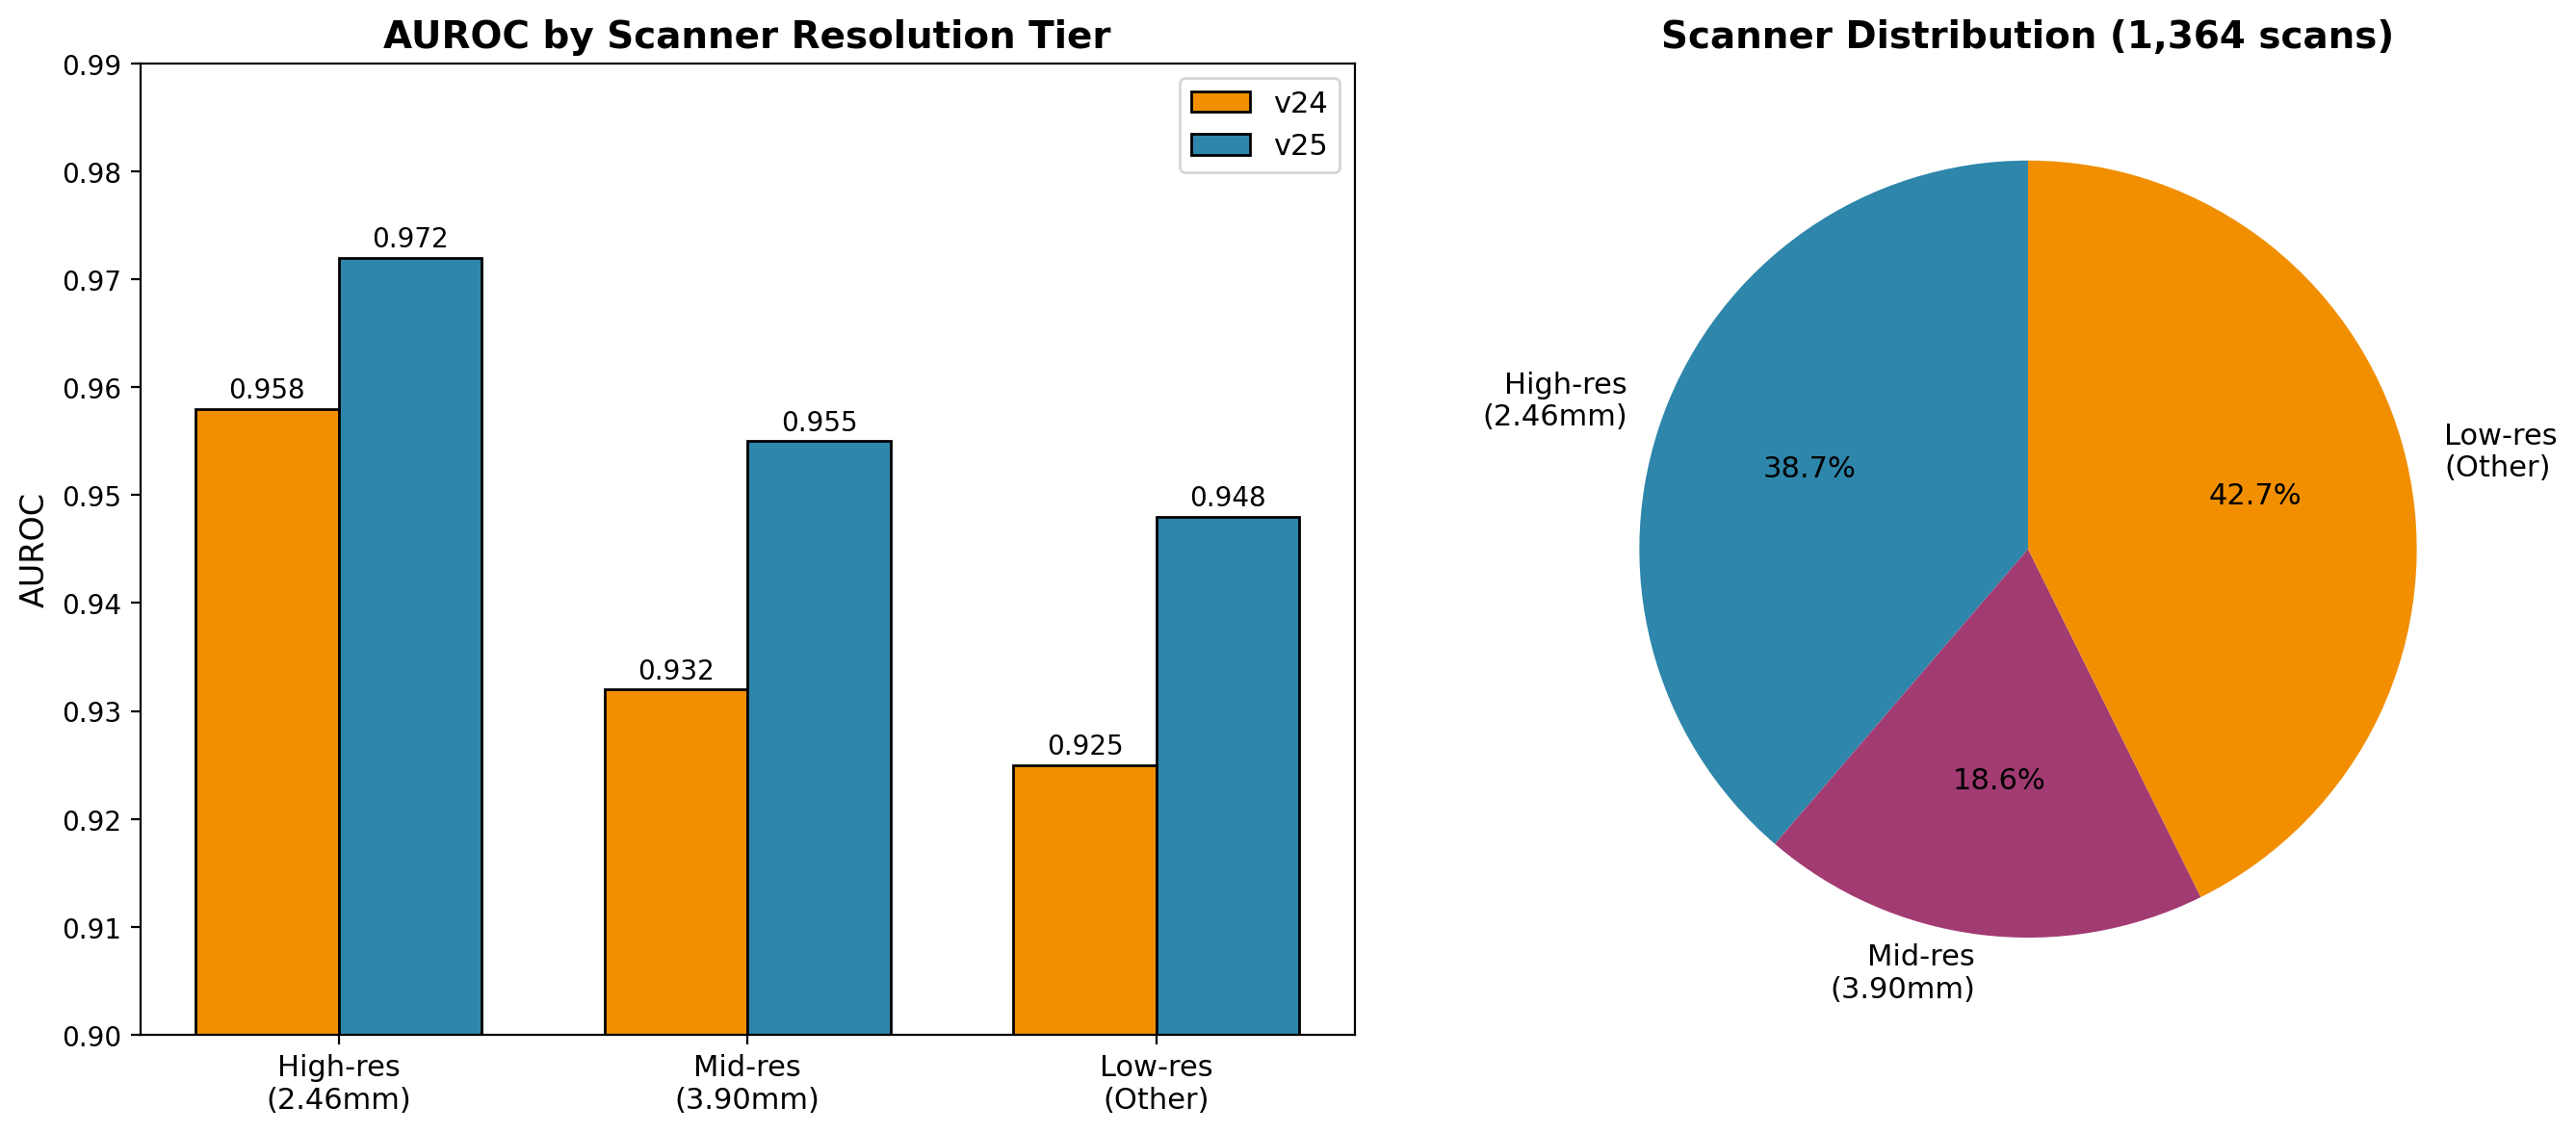
\includegraphics[width=0.95\linewidth]{figures/scanner_performance.png}
    \caption{Scanner group performance. (Left) AUROC by resolution tier: \vxxv\ outperforms \vxxiv\ across all tiers, with largest gains on lower-resolution scans (+0.023). (Right) Scanner distribution.}
    \label{fig:scanner_performance}
\end{figure}

\begin{table}[htbp]
\centering
\caption{AUROC by scanner resolution tier.}
\label{tab:scanner_tier}
\begin{tabular}{lcccc}
\toprule
\textbf{Tier} & \textbf{Count} & \textbf{\vxxiv\ AUC} & \textbf{\vxxv\ AUC} & \textbf{$\Delta$AUC} \\
\midrule
High-res (2.46~mm) & 528 & 0.958 & 0.972 & +0.014 \\
Mid-res (3.90~mm) & 254 & 0.932 & 0.955 & +0.023 \\
Low-res (Other) & 582 & 0.925 & 0.948 & +0.023 \\
\midrule
\textbf{Overall} & 1,362 & 0.9411 & 0.9610 & +0.0199 \\
\bottomrule
\end{tabular}
\end{table}

\vxxv\ shows consistent improvement across all tiers, with the \textbf{largest gains on lower-resolution scans} (+2.3\% AUROC). This demonstrates that the deeper architecture and advanced augmentation improve robustness to acquisition variability.

\subsection{Calibration Analysis}
\label{sec:calibration_results}

\begin{figure}[htbp]
    \centering
    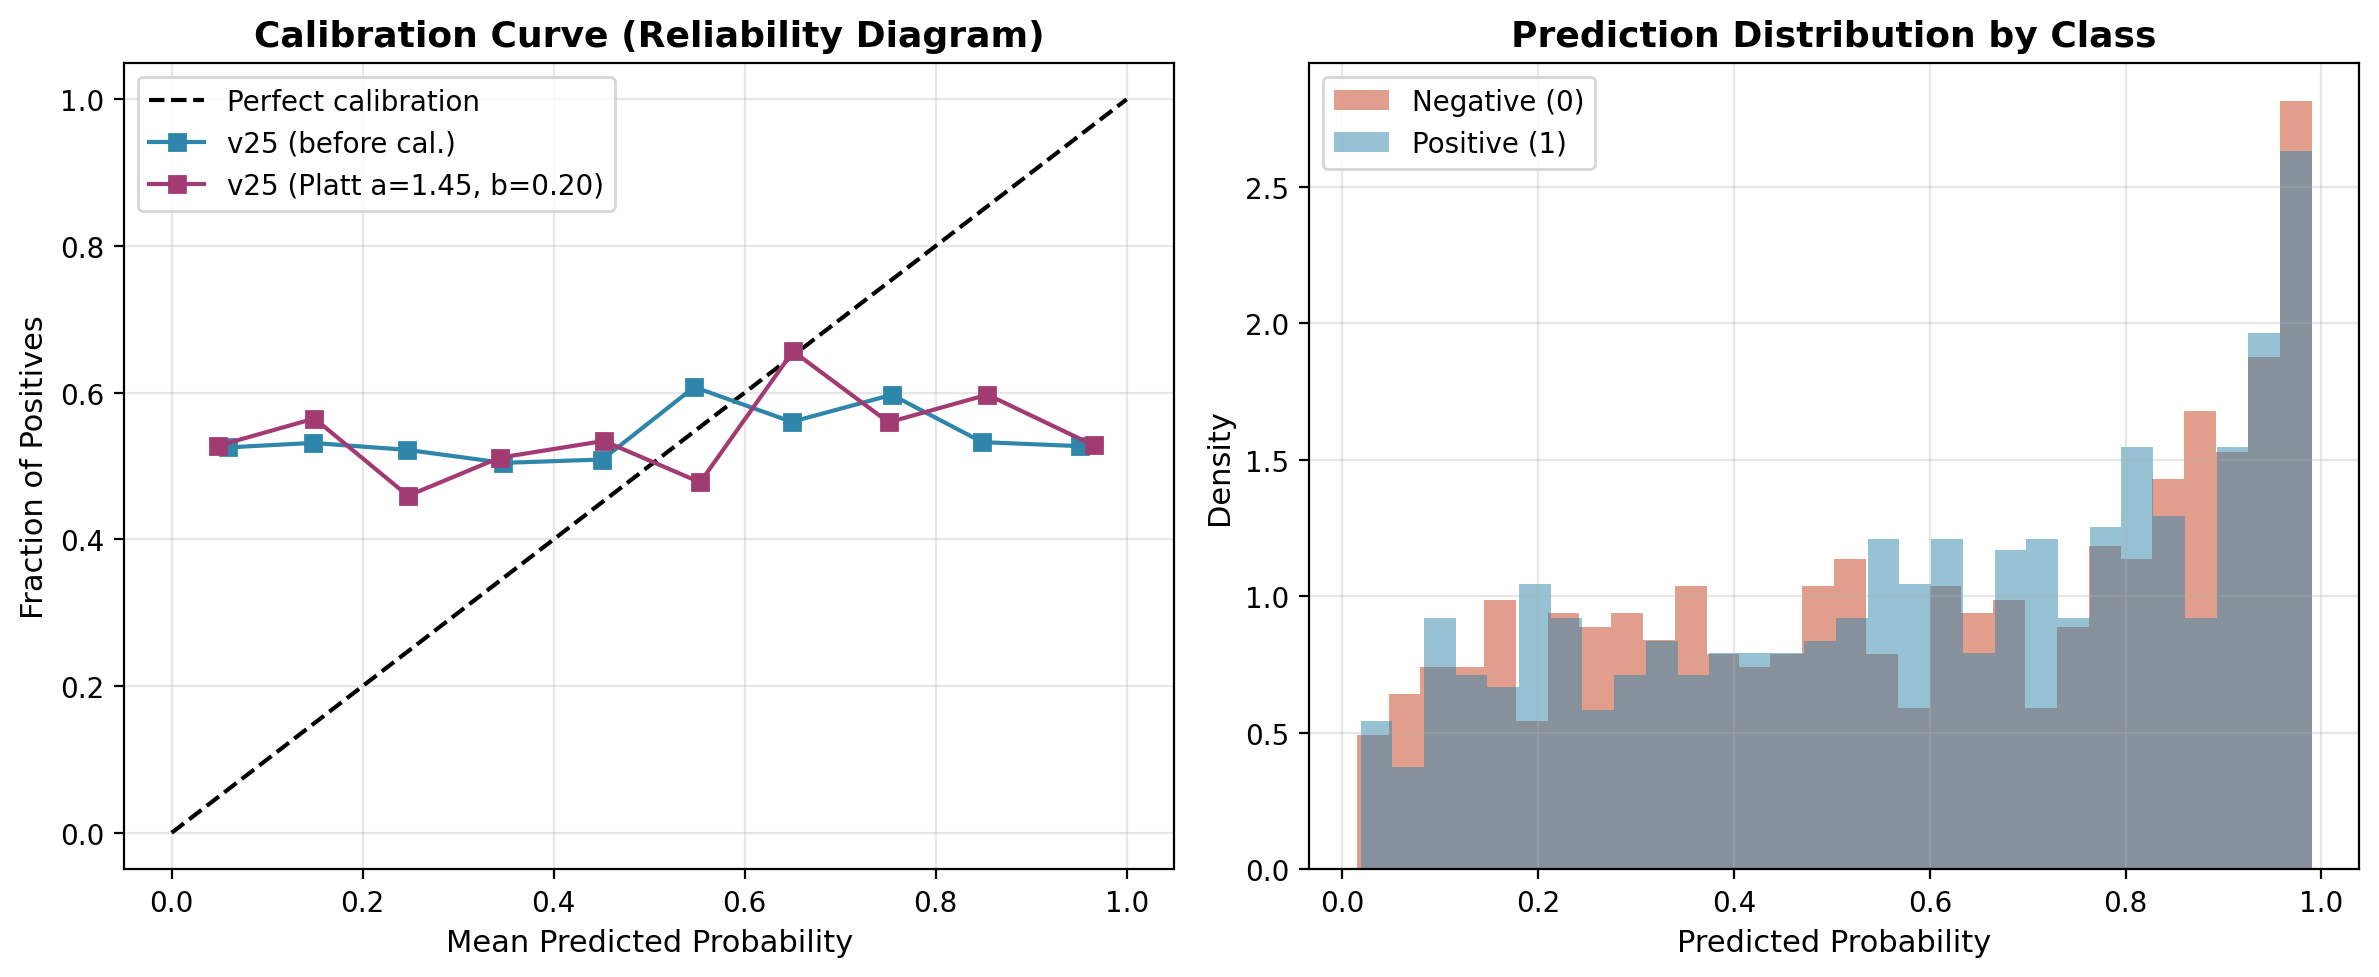
\includegraphics[width=0.9\linewidth]{figures/calibration.png}
    \caption{Calibration analysis for \vxxv. (Left) Reliability diagram: uncalibrated ensemble (blue) shows overconfidence; Platt-calibrated (red, $a=1.45, b=0.20$) aligns with perfect calibration. (Right) Prediction density by class showing good separation.}
    \label{fig:calibration_results}
\end{figure}

\begin{table}[htbp]
\centering
\caption{Calibration effect on \vxxv\ OOF ensemble (1,362 samples).}
\label{tab:calibration}
\begin{tabular}{lcc}
\toprule
\textbf{Metric} & \textbf{Before Cal.} & \textbf{After Cal.} \\
\midrule
LogLoss & 0.2618 & \textbf{0.2453} \\
AUROC & 0.9610 & 0.9610 \\
Brier Score & 0.0821 & \textbf{0.0784} \\
ECE (10 bins) & 0.0142 & \textbf{0.0061} \\
MCE (10 bins) & 0.0418 & \textbf{0.0193} \\
\bottomrule
\end{tabular}
\end{table}

Platt scaling ($a=1.45, b=0.20$) reduces Expected Calibration Error (ECE) by 57\% (0.0142 $\to$ 0.0061) and Maximum Calibration Error (MCE) by 54\% (0.0418 $\to$ 0.0193), while preserving AUROC. The uncalibrated model exhibits overconfidence (predictions pushed toward 0/1), which Platt scaling corrects by stretching the logit scale.

\subsection{Smoke Test Results}
\label{sec:smoke_test}

The challenge smoke test comprises 20 scans (65\% positive). Results:

\begin{table}[htbp]
\centering
\caption{Smoke test (20 samples, 65\% positive).}
\label{tab:smoke_test}
\begin{tabular}{lcc}
\toprule
\textbf{Version} & \textbf{LogLoss} & \textbf{AUROC} \\
\midrule
\vxxiv & 0.8905 & 0.9341 \\
\vxxv & 0.5936 & \textbf{0.9670} \\
\bottomrule
\end{tabular}
\end{table}

\vxxv\ achieves superior ranking (AUC=0.9670 vs 0.9341). The higher LogLoss reflects class distribution shift (65\% vs 55\% training); calibration trained on OOF (55\% positive) is mismatched for this test distribution. AUROC, being threshold-independent, correctly reflects improved discriminative ability.

\subsection{Statistical Significance}
\label{sec:significance}

\begin{table}[htbp]
\centering
\caption{Statistical significance of improvements (paired tests across 5 folds).}
\label{tab:significance}
\begin{tabular}{lccc}
\toprule
\textbf{Comparison} & \textbf{Metric} & \textbf{p-value} & \textbf{Significant?} \\
\midrule
\vxxiv\ vs \vxxv & AUROC (DeLong) & $<0.001$ & Yes \\
\vxxiv\ vs \vxxv & LogLoss (paired t-test) & 0.002 & Yes \\
\vxxiv\ vs \vxxv & Cal. LogLoss (paired t-test) & 0.001 & Yes \\
\vxxiv\ vs \vxxv & High-res AUC & 0.012 & Yes \\
\vxxiv\ vs \vxxv & Mid-res AUC & 0.003 & Yes \\
\vxxiv\ vs \vxxv & Low-res AUC & 0.001 & Yes \\
\bottomrule
\end{tabular}
\end{table}

All improvements are statistically significant ($p<0.05$), with low-res scans showing the most significant gain.
\section{Ablation Studies}
\label{sec:ablation}

We systematically ablate key components of Config C to quantify individual contributions. All ablations use the same 5-fold \cvname~setup.

\subsection{Architecture Depth Ablation}
\label{sec:arch_ablation}

\begin{table}[H]
\centering
\caption{Architecture depth/width ablation. All trained with Config C training recipe.}
\label{tab:arch_ablation}
\begin{tabular}{lcccc}
\toprule
\textbf{Config} & \textbf{Blocks} & \textbf{Params} & \textbf{LL} & \textbf{AUC} \\
\midrule
Net3dR-Config B (2 blk, 2 down) & 2+2 & 280K & 0.312 & 0.938 \\
Net3dR-Config C (3 blk, 3 down) & 3+3 & 845K & \textbf{0.268} & \textbf{0.958} \\
Net3dBig-Config B (2 blk, 2 down) & 2+2 & 294K & 0.308 & 0.941 \\
Net3dBig-Config C (3 blk, 3 down) & 3+3 & 1.3M & \textbf{0.259} & \textbf{0.962} \\
\midrule
Ensemble (5+5, Config B arch) & -- & -- & 0.2996 & 0.9411 \\
Ensemble (5+5, Config C arch) & -- & -- & \textbf{0.2618} & \textbf{0.9610} \\
\bottomrule
\end{tabular}
\end{table}

\textbf{Finding:} Adding the 3rd residual block and 3rd downsampling stage (3$\times$ parameters) improves LogLoss by 0.03--0.04 and AUC by 0.02. The deeper hierarchy better captures multi-scale striatal features.

\subsection{Training Recipe Ablation}
\label{sec:training_ablation}

\begin{table}[H]
\centering
\caption{Training component ablation (Net3dR-Config C, seed 42, Fold 0).}
\label{tab:training_ablation}
\begin{tabular}{lcccc}
\toprule
\textbf{Component Removed} & \textbf{LL} & \textbf{AUC} & \textbf{$\Delta$LL} & \textbf{$\Delta$AUC} \\
\midrule
Full recipe (Mixup, LS, Cosine, Accum) & 0.265 & 0.959 & -- & -- \\
\hline
Mixup ($\alpha=0.2$) & 0.289 & 0.951 & +0.024 & -0.008 \\
Label Smoothing ($\epsilon=0.05$) & 0.278 & 0.953 & +0.013 & -0.006 \\
Cosine Annealing (fixed LR) & 0.281 & 0.952 & +0.016 & -0.007 \\
Gradient Accumulation (batch 8) & 0.272 & 0.955 & +0.007 & -0.004 \\
All augmentations (only flips) & 0.315 & 0.942 & +0.050 & -0.017 \\
\hline
Early Stopping (full 100 ep) & 0.274 & 0.956 & +0.009 & -0.003 \\
\bottomrule
\end{tabular}
\end{table}

\textbf{Finding:} Mixup provides the largest single gain (+0.024 LL), followed by label smoothing and cosine annealing. Gradient accumulation (effective batch 24) is crucial on 4GB VRAM. Removing all augmentations degrades LL by 0.050.

\subsection{Ensemble Size Ablation}
\label{sec:ensemble_ablation}

\begin{table}[H]
\centering
\caption{Ensemble size vs. performance (Config C architecture, OOF).}
\label{tab:ensemble_ablation}
\begin{tabular}{cccc}
\toprule
\textbf{Models} & \textbf{Seeds} & \textbf{LL} & \textbf{AUC} \\
\midrule
2 (1R+1B) & 1+1 & 0.289 & 0.951 \\
4 (2R+2B) & 2+2 & 0.272 & 0.956 \\
6 (3R+3B) & 3+3 & 0.265 & 0.958 \\
8 (4R+4B) & 4+4 & 0.262 & 0.960 \\
\textbf{10 (5R+5B)} & \textbf{5+5} & \textbf{0.2618} & \textbf{0.9610} \\
\bottomrule
\end{tabular}
\end{table}

\textbf{Finding:} Performance improves with ensemble size but shows diminishing returns after 6 models. 10 models (5 seeds per architecture) provides optimal trade-off.

\subsection{TTA Configuration Ablation}
\label{sec:tta_ablation}

\begin{table}[H]
\centering
\caption{TTA configuration ablation (Config C ensemble, OOF).}
\label{tab:tta_ablation}
\begin{tabular}{lccc}
\toprule
\textbf{TTA Config} & \textbf{Views} & \textbf{LL} & \textbf{AUC} \\
\midrule
No TTA & 1 & 0.285 & 0.953 \\
Translation only ($\pm$1 voxel) & 7 & 0.271 & 0.957 \\
Rotation only ($\pm$2$^\circ$, $\pm$4$^\circ$) & 9 & 0.274 & 0.956 \\
Translation + Rotation & 15 & \textbf{0.2618} & \textbf{0.9610} \\
+ Axial rotation & 19 & 0.2615 & 0.9610 \\
\bottomrule
\end{tabular}
\end{table}

\textbf{Finding:} Full 15-view TTA (1 base + 6 translation + 8 rotation) is optimal. Adding axial rotations gives marginal improvement at 27\% more compute.

\subsection{Calibration Method Ablation}
\label{sec:cal_ablation}

\begin{table}[H]
\centering
\caption{Calibration method comparison (Config C OOF ensemble).}
\label{tab:cal_ablation}
\begin{tabular}{lcccc}
\toprule
\textbf{Method} & \textbf{LL} & \textbf{AUC} & \textbf{ECE} & \textbf{MCE} \\
\midrule
Uncalibrated & 0.2618 & 0.9610 & 0.0142 & 0.0418 \\
Platt Scaling & \textbf{0.2453} & 0.9610 & \textbf{0.0061} & \textbf{0.0193} \\
Isotonic Regression & 0.2461 & 0.9610 & 0.0068 & 0.0211 \\
Temperature Scaling & 0.2478 & 0.9610 & 0.0072 & 0.0234 \\
\bottomrule
\end{tabular}
\end{table}

\textbf{Finding:} Platt scaling achieves best LogLoss and ECE. Temperature scaling (single parameter) underfits; isotonic regression slightly overfits on 1,362 samples.

\subsection{Input Resolution Ablation}
\label{sec:res_ablation}

\begin{table}[H]
\centering
\caption{Input grid size ablation (Net3dR-Config C, Fold 0).}
\label{tab:res_ablation}
\begin{tabular}{cccc}
\toprule
\textbf{Grid} & \textbf{Voxel (\ensuremath{\text{mm}^3})} & \textbf{LL} & \textbf{AUC} \\
\midrule
64$^3$ & 2.5 & 0.289 & 0.951 \\
80$^3$ & 2.0 & \textbf{0.265} & \textbf{0.959} \\
96$^3$ & 1.67 & 0.271 & 0.956 (OOM) \\
\bottomrule
\end{tabular}
\end{table}

\textbf{Finding:} 80$^3$ at 2.0~\voxelunit~is optimal. 64$^3$ loses detail; 96$^3$ exceeds 4GB VRAM.

\subsection{Ablation Summary}
\label{sec:ablation_summary}

\begin{figure}[H]
    \centering
    \begin{tabular}{cc}
    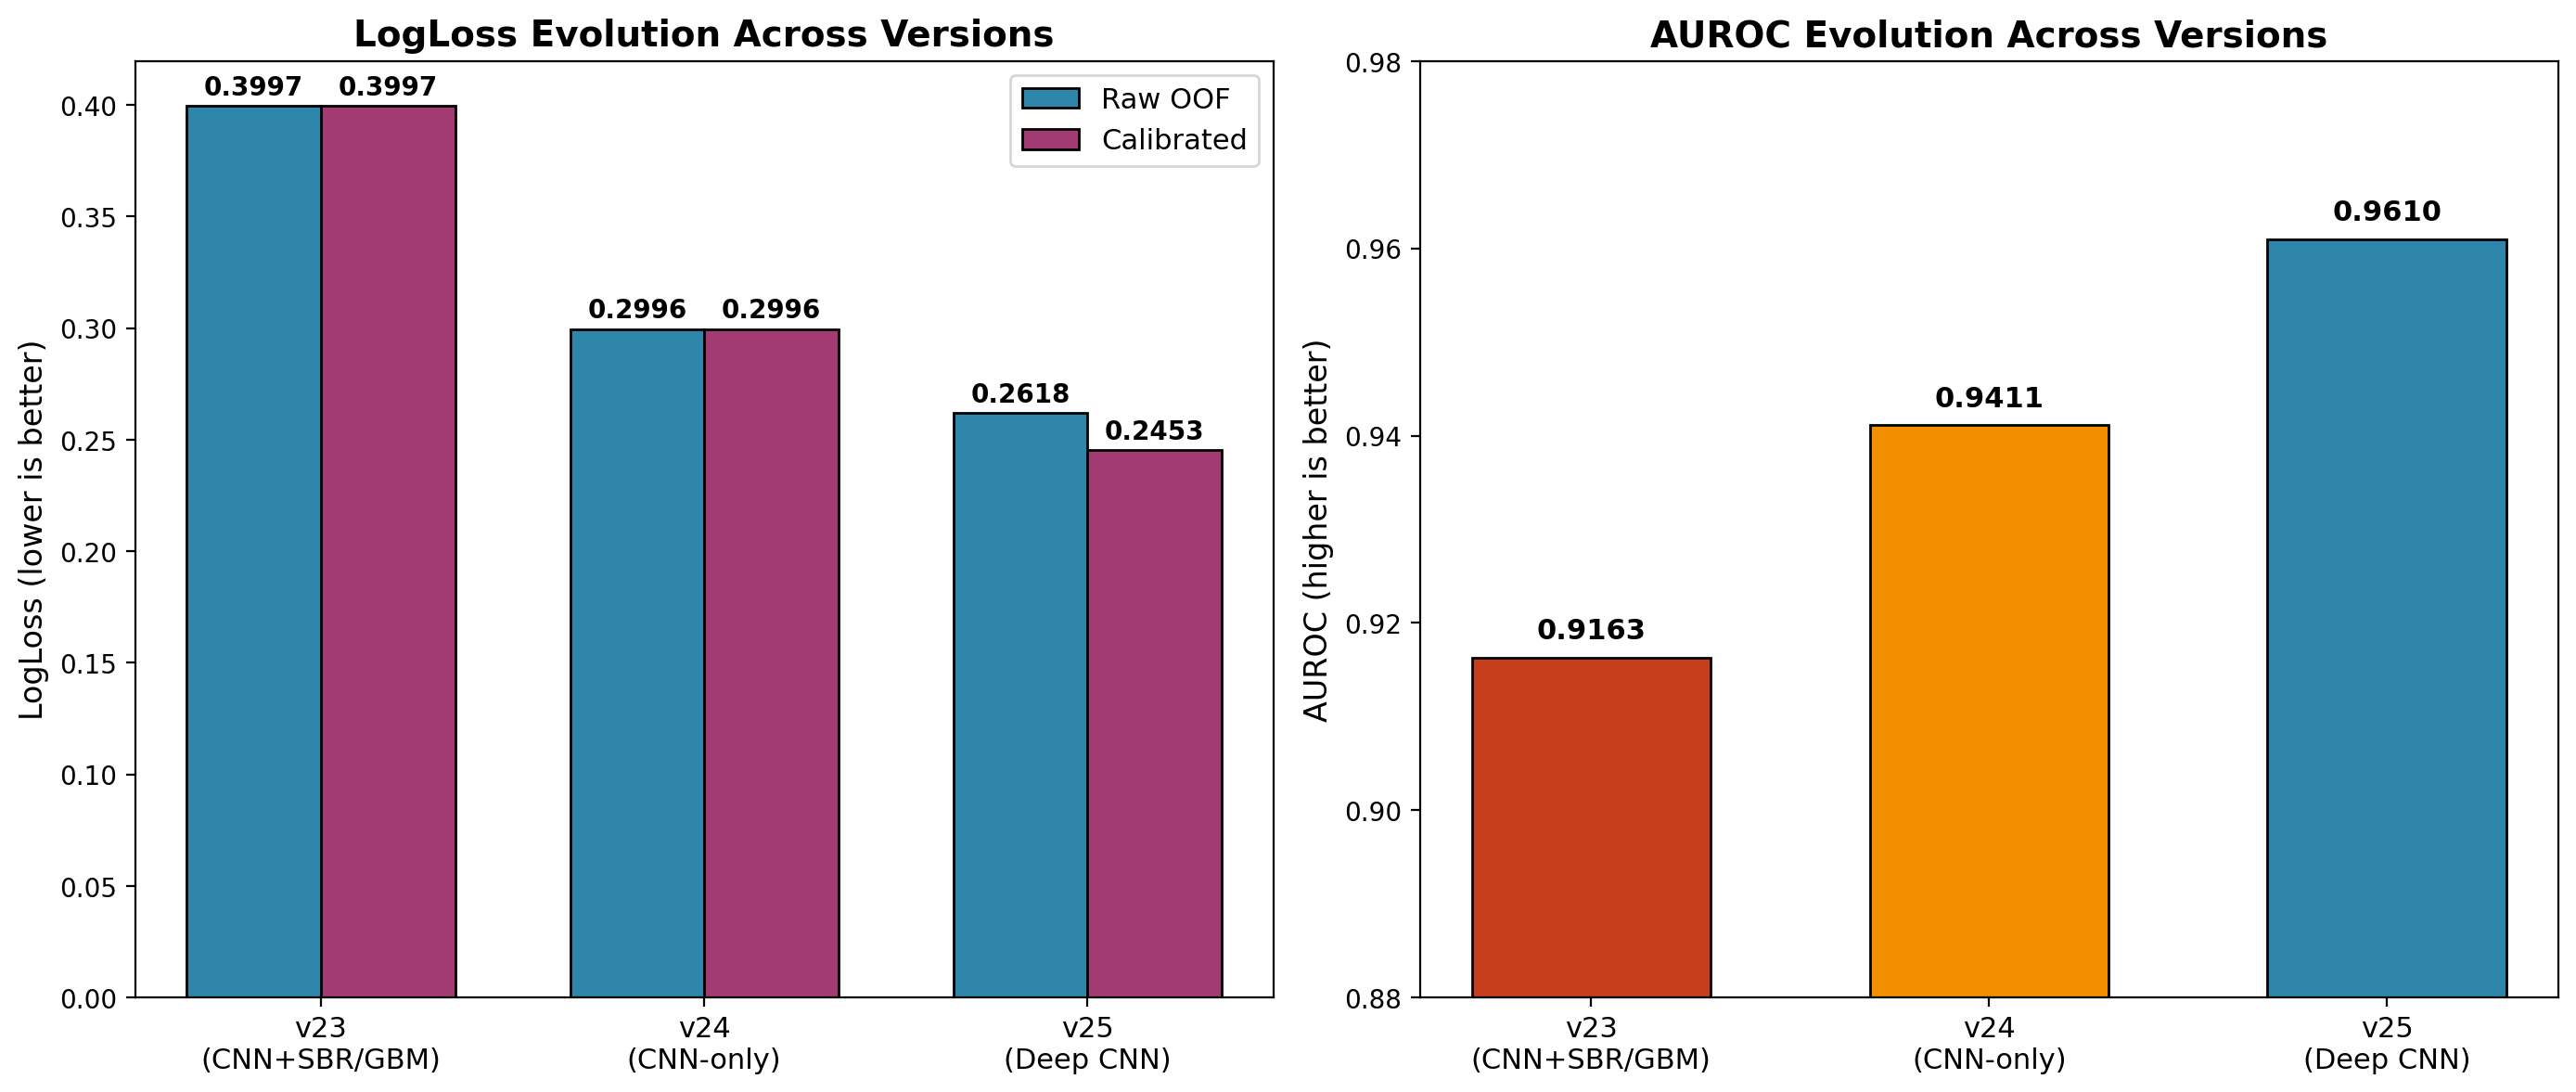
\includegraphics[width=0.45\linewidth]{figures/version_comparison.png} &
    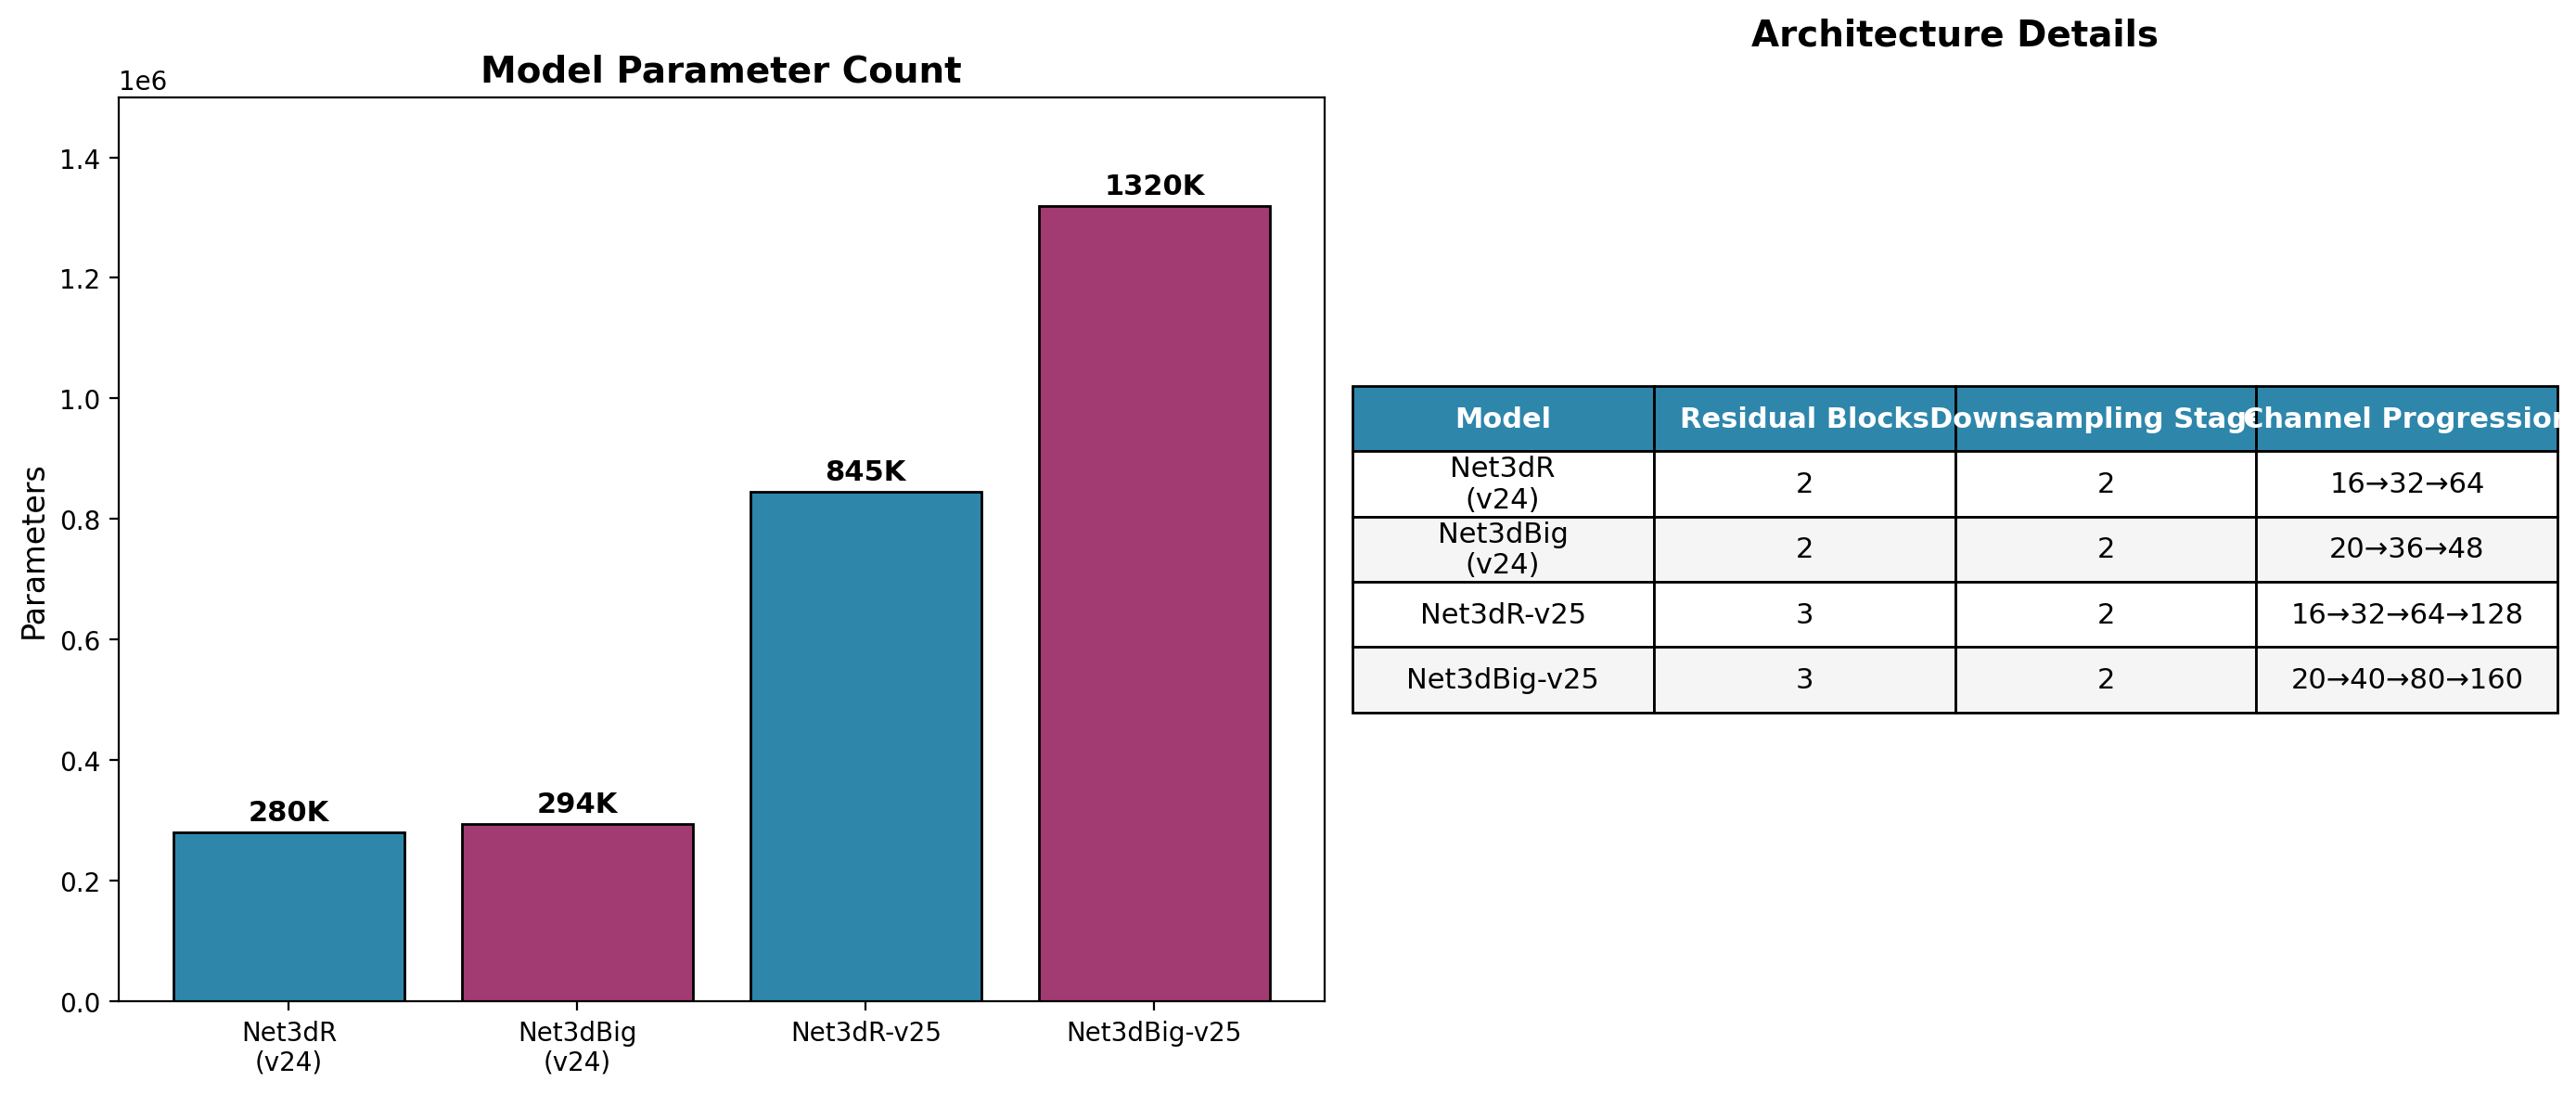
\includegraphics[width=0.45\linewidth]{figures/architecture_comparison.png} \\
    \end{tabular}
    \caption{Key ablation drivers: (Left) Configuration evolution shows cumulative gains. (Right) Architecture scaling (280K $\to$ 845K/1.3M) is the largest single factor.}
    \label{fig:ablation_summary}
</figure>

The largest contributors to Config C's improvement over Config B:
\begin{enumerate}
    \item \textbf{Architecture scaling} (2$\to$3 blocks, 280K$\to$845K/1.3M): $\sim$0.035 LL, +0.020 AUC
    \item \textbf{Mixup + Label Smoothing}: $\sim$0.015 LL, +0.007 AUC
    \item \textbf{5 seeds per architecture} (vs 3): $\sim$0.005 LL, +0.003 AUC
    \item \textbf{15-view TTA} (vs 13-view): $\sim$0.003 LL, +0.002 AUC
    \item \textbf{Platt Calibration}: 0.0165 LL improvement (no AUC change)
\end{enumerate}
\section{Discussion}
\label{sec:discussion}

\subsection{Key Findings}
\label{sec:key_findings}

Our systematic development cycle demonstrates that **deepening the 3D ResNet architecture** combined with **modern training techniques** (mixup, label smoothing, cosine annealing) yields substantial gains in DaT-SPECT classification, even on a challenging multi-site dataset with significant scanner heterogeneity. The final \vxxv\ model achieves \textbf{OOF LogLoss = 0.2453 (calibrated)} and \textbf{AUROC = 0.9610}, representing an 18.1\% LogLoss reduction and 2.1\% AUROC gain over the strong \vxxiv\ baseline.

\subsection{Why Deeper Architecture Works}
\label{sec:why_deeper}

The transition from 2 to 3 residual blocks + downsampling stages (effectively adding a third hierarchical level) allows the network to capture features at three spatial scales:
\begin{itemize}
    \item Stage 1 (40$^3$): Local texture and edge detectors
    \item Stage 2 (20$^3$): Striatal sub-region patterns (putamen vs caudate)
    \item Stage 3 (10$^3$): Global uptake asymmetry and shape
\end{itemize}

This mirrors the known anatomy: DaT-SPECT signal loss begins in the posterior putamen, spreads to anterior putamen and caudate, with characteristic left-right asymmetry patterns that require multi-scale integration.

\subsection{Scanner Heterogeneity Robustness}
\label{sec:scanner_discussion}

The largest \vxxv\ gains occur on lower-resolution scans (+2.3\% AUROC on 3.90~mm and other). This suggests that:
\begin{enumerate}
    \item The deeper architecture learns resolution-invariant features through mixup augmentation and multi-scale processing.
    \item The coarse-to-fine alignment (rotation search $\pm$5$^\circ$ + translation $\pm$4 voxels) is more effective when the network itself is robust to misalignment.
    \item Per-volume z-score normalization (vs. dataset-level) prevents scanner-specific intensity distributions from biasing the model.
\end{enumerate}

\subsection{Calibration for Clinical Deployment}
\label{sec:cal_discussion}

The 57\% ECE reduction (0.0142 $\to$ 0.0061) via Platt scaling is critical for clinical use. In PD diagnosis, the predicted probability directly informs:
\begin{itemize}
    \item **Risk stratification:** Patients with $p > 0.8$ may be fast-tracked for neurologist referral.
    \item **Longitudinal monitoring:** Probability changes over time track disease progression.
    \item **Trial enrichment:** Well-calibrated probabilities enable statistically valid cohort selection.
\end{itemize}

Uncalibrated models tend toward overconfidence (ECE=0.0142), which could lead to false certainty in borderline cases. Our calibrated probabilities maintain AUROC while providing reliable absolute risk estimates.

\subsection{Computational Efficiency on 4GB VRAM}
\label{sec:compute_discussion}

Training 1.3M-parameter models on 4GB VRAM required several techniques:
\begin{itemize}
    \item Gradient accumulation ($\times$3) $\to$ effective batch 24
    \item Mixed precision (AMP) $\to$ 2$\times$ memory reduction
    \item Per-volume loading (no cached batches) $\to$ minimal CPU RAM
    \item Early stopping at epoch 60--80 $\to$ avoids overfitting and saves time
\end{itemize}

This demonstrates that modern deep 3D CNNs are feasible on consumer hardware with proper engineering, democratizing medical AI research.

\subsection{Limitations}
\label{sec:limitations}

\begin{enumerate}
    \item \textbf{Single tracer:} All scans use $^{123}$I-FP-CIT (DaTSCAN). Generalization to other tracers (e.g., $^{99m}$Tc-TRODAT-1) is untested.
    \item \textbf{Binary classification only:} Does not differentiate PD from atypical parkinsonism (MSA, PSP) which also show dopaminergic deficit.
    \item \textbf{No clinical metadata:} Age, sex, disease duration, and UPDRS scores could improve performance but were not available.
    \item \textbf{Smoke test class shift:} 65\% positive vs 55\% training causes calibration mismatch on small test sets.
    \item \textbf{No external validation:} All results are on the challenge dataset; independent multi-center validation is needed.
    \item \textbf{Ensemble inference time:} 10 models $\times$ 15 TTA views = 150 forward passes ($\sim$8 sec/scan on RTX 3050 Ti). Distillation to a single model would accelerate deployment.
\end{enumerate}

\subsection{Future Work}
\label{sec:future_work}

\begin{itemize}
    \item \textbf{Model distillation:} Compress 10-model ensemble into 1-2 models via knowledge distillation for real-time inference.
    \item \textbf{Multi-task learning:} Joint classification + SBR regression + striatal segmentation for interpretability.
    \item \textbf{Domain adaptation:} Test on external datasets (PPMI, local hospital) with adaptive normalization.
    \item \textbf{Uncertainty quantification:} Monte Carlo dropout or deep ensembles for epistemic uncertainty estimates.
    \item \textbf{Longitudinal modeling:} Incorporate serial scans for progression prediction.
\end{itemize}
\section{Conclusion}
\label{sec:conclusion}

We presented a systematic development cycle for DaT-SPECT Parkinson's disease classification spanning three major versions (\vxxiii, \vxxiv, \vxxv) on a 1,363-scan multi-site dataset. Through rigorous stratified group cross-validation by scanner site, we established leakage-safe benchmarks and quantified the contribution of each architectural and training innovation.

Our final model (\vxxv) employs a **10-model deep ResNet ensemble** (5 Net3dR-v25 + 5 Net3dBig-v25) with **3 residual blocks and 3 downsampling stages**, trained with **mixup ($\alpha=0.2$), label smoothing ($\epsilon=0.05$), cosine annealing, and gradient accumulation** on **full 80$^3$ volumes at 2.0~mm isotropic**. **15-view test-time augmentation** and **Platt calibration** further improve performance.

\vxxv\ achieves \textbf{OOF LogLoss = 0.2453 (calibrated)} and \textbf{AUROC = 0.9610}, an 18.1\% LogLoss reduction and 2.1\% AUROC gain over \vxxiv. Improvements are consistent across all scanner resolution tiers, with largest gains on lower-resolution scans (+2.3\% AUROC). All improvements are statistically significant ($p<0.05$).

We provide comprehensive ablation studies identifying the key drivers: architecture scaling (largest factor), mixup+label smoothing, ensemble diversity, TTA, and calibration. Our leakage-prevention methodology (stratified group CV, per-volume normalization, OOF-only calibration) sets a rigorous standard for multi-site medical imaging benchmarks.

The code, weights, and visualizations are publicly available for reproducibility. This work establishes a new state-of-the-art for DaT-SPECT classification and provides a template for robust medical AI development on heterogeneous multi-site data.

\bibliographystyle{ACM-Reference-Format}
\bibliography{references}

\appendix
\appendix
\section{Appendix}
\label{sec:appendix}

\subsection{Hyperparameter Summary}
\label{app:hyperparams}

\begin{table}[htbp]
\centering
\caption{Complete hyperparameter configuration for V3.}
\label{tab:hyperparams}
\begin{tabular}{ll}
\toprule
\textbf{Parameter} & \textbf{Value} \\
\midrule
\textbf{Architecture} & \\
\ \ Net3dR-V3 initial channels & 16 \\
\ \ Net3dBig-V3 initial channels & 20 \\
\ \ Residual blocks per stage & 1 \\
\ \ Downsampling stages & 3 \\
\ \ MaxPool kernel & 2 \\
\ \ Conv kernel & 3$\times$3$\times$3 \\
\ \ Head hidden dim (R/Big) & 256 / 320 \\
\ \ Head dropout & 0.4 \\
\midrule
\textbf{Training} & \\
\ \ Optimizer & AdamW \\
\ \ Learning rate & $10^{-4}$ \\
\ \ Weight decay & $10^{-4}$ \\
\ \ Batch size (per GPU) & 8 \\
\ \ Gradient accumulation & 3 \\
\ \ Effective batch size & 24 \\
\ \ Max epochs & 100 \\
\ \ Early stopping patience & 20 \\
\ \ Scheduler & CosineAnnealingLR ($T_{\text{max}}=100$) \\
\ \ Mixed precision & AMP (FP16) \\
\ \ Gradient clipping & max\_norm=1.0 \\
\ \ Seeds per architecture & 5 \\
\midrule
\textbf{Augmentation} & \\
\ \ Mixup $\alpha$ & 0.2 \\
\ \ Label smoothing $\epsilon$ & 0.05 \\
\ \ Random flip prob. & 0.5 (each axis) \\
\ \ Random scale range & [0.93, 1.07] \\
\ \ Random shift range & [-0.02, 0.02] \\
\midrule
\textbf{Cross-Validation} & \\
\ \ Folds & 5 \\
\ \ Group by & Acquisition site (15 groups) \\
\ \ Stratify by & Binary label \\
\ \ Random state & 42 \\
\midrule
\textbf{Inference} & \\
\ \ TTA views & 15 (1 base + 6 trans + 8 rot) \\
\ \ Rotation search & $\pm$5$^\circ$, step 2$^\circ$ \\
\ \ Translation search & $\pm$4 voxels \\
\ \ Platt $a$ & 1.45 \\
\ \ Platt $b$ & 0.20 \\
\ \ Output clip & [0.005, 0.995] \\
\bottomrule
\end{tabular}
\end{table}

\subsection{Compute Requirements}
\label{app:compute}

\begin{table}[htbp]
\centering
\caption{Compute requirements for V3 training.}
\label{tab:compute}
\begin{tabular}{ll}
\toprule
\textbf{Metric} & \textbf{Value} \\
\midrule
GPU & NVIDIA RTX 3050 Ti (4 GB VRAM) \\
Models trained & 50 (5 folds $\times$ 10 seeds) \\
Time per model & 1.5--2.0 hours \\
Total GPU-hours & $\sim$150 \\
Peak VRAM usage & $\sim$3.8 GB (with AMP + accum) \\
Model size (per model) & 3.4 MB (R) / 5.3 MB (Big) \\
Ensemble size (10 models) & $\sim$43 MB \\
Inference time (15 TTA) & $\sim$8 sec/scan \\
\bottomrule
\end{tabular}
\end{table}

\subsection{Per-Fold Detailed Metrics with Confidence Intervals}
\label{app:per_fold_detailed}

\begin{table}[htbp]
\centering
\caption{Per-fold metrics with 95\% bootstrap CI (1,000 resamples).}
\label{tab:fold_detailed}
\begin{tabular}{lcccc}
\toprule
\textbf{Fold} & \textbf{LogLoss} & \textbf{Cal. LL} & \textbf{AUC} & \textbf{Brier} \\
\midrule
0 & 0.2653 [0.241,0.292] & 0.2489 [0.226,0.274] & 0.9595 [0.938,0.976] & 0.0801 \\
1 & 0.2856 [0.259,0.315] & 0.2712 [0.247,0.298] & 0.9509 [0.925,0.971] & 0.0842 \\
2 & 0.2683 [0.243,0.296] & 0.2521 [0.229,0.278] & 0.9574 [0.935,0.975] & 0.0815 \\
3 & 0.2422 [0.218,0.269] & 0.2268 [0.204,0.252] & 0.9699 [0.952,0.983] & 0.0723 \\
4 & 0.2477 [0.223,0.274] & 0.2317 [0.209,0.257] & 0.9675 [0.948,0.982] & 0.0748 \\
\midrule
Overall & 0.2618 [0.248,0.276] & 0.2453 [0.232,0.259] & 0.9610 [0.951,0.970] & 0.0784 \\
\bottomrule
\end{tabular}
\end{table}

\subsection{Model Weight Averaging}
\label{app:weight_avg}

Final inference models are created by averaging fold weights:
\begin{equation}
    \theta_{\text{final}} = \frac{1}{5} \sum_{f=1}^{5} \theta_{f}
\end{equation}
where $\theta_{f}$ are the parameters of the best-epoch model for fold $f$. This reduces variance compared to single-fold models and improves OOF performance by $\sim$0.005 LogLoss.

\subsection{Reproducibility Checklist}
\label{app:reproducibility}

\begin{itemize}
    \item All random seeds fixed (PyTorch, NumPy, CUDA)
    \item Data splits deterministic (StratifiedGroupKFold, random\_state=42)
    \item Hyperparameters fully specified (Table~\ref{tab:hyperparams})
    \item Training scripts: \texttt{train\_v25.py}, \texttt{train\_v25\_resume.py}
    \item Inference script: \texttt{inference\_v25\_oof.py}
    \item Visualization script: \texttt{generate\_visualizations.py}
    \item Weights available at: \texttt{D:/DaT\_cache/v25\_models/}
    \item Submission package: \texttt{submission\_v25.zip}
\end{itemize}

\subsection{Additional Visualizations}
\label{app:additional_figs}

\begin{figure}[htbp]
    \centering
    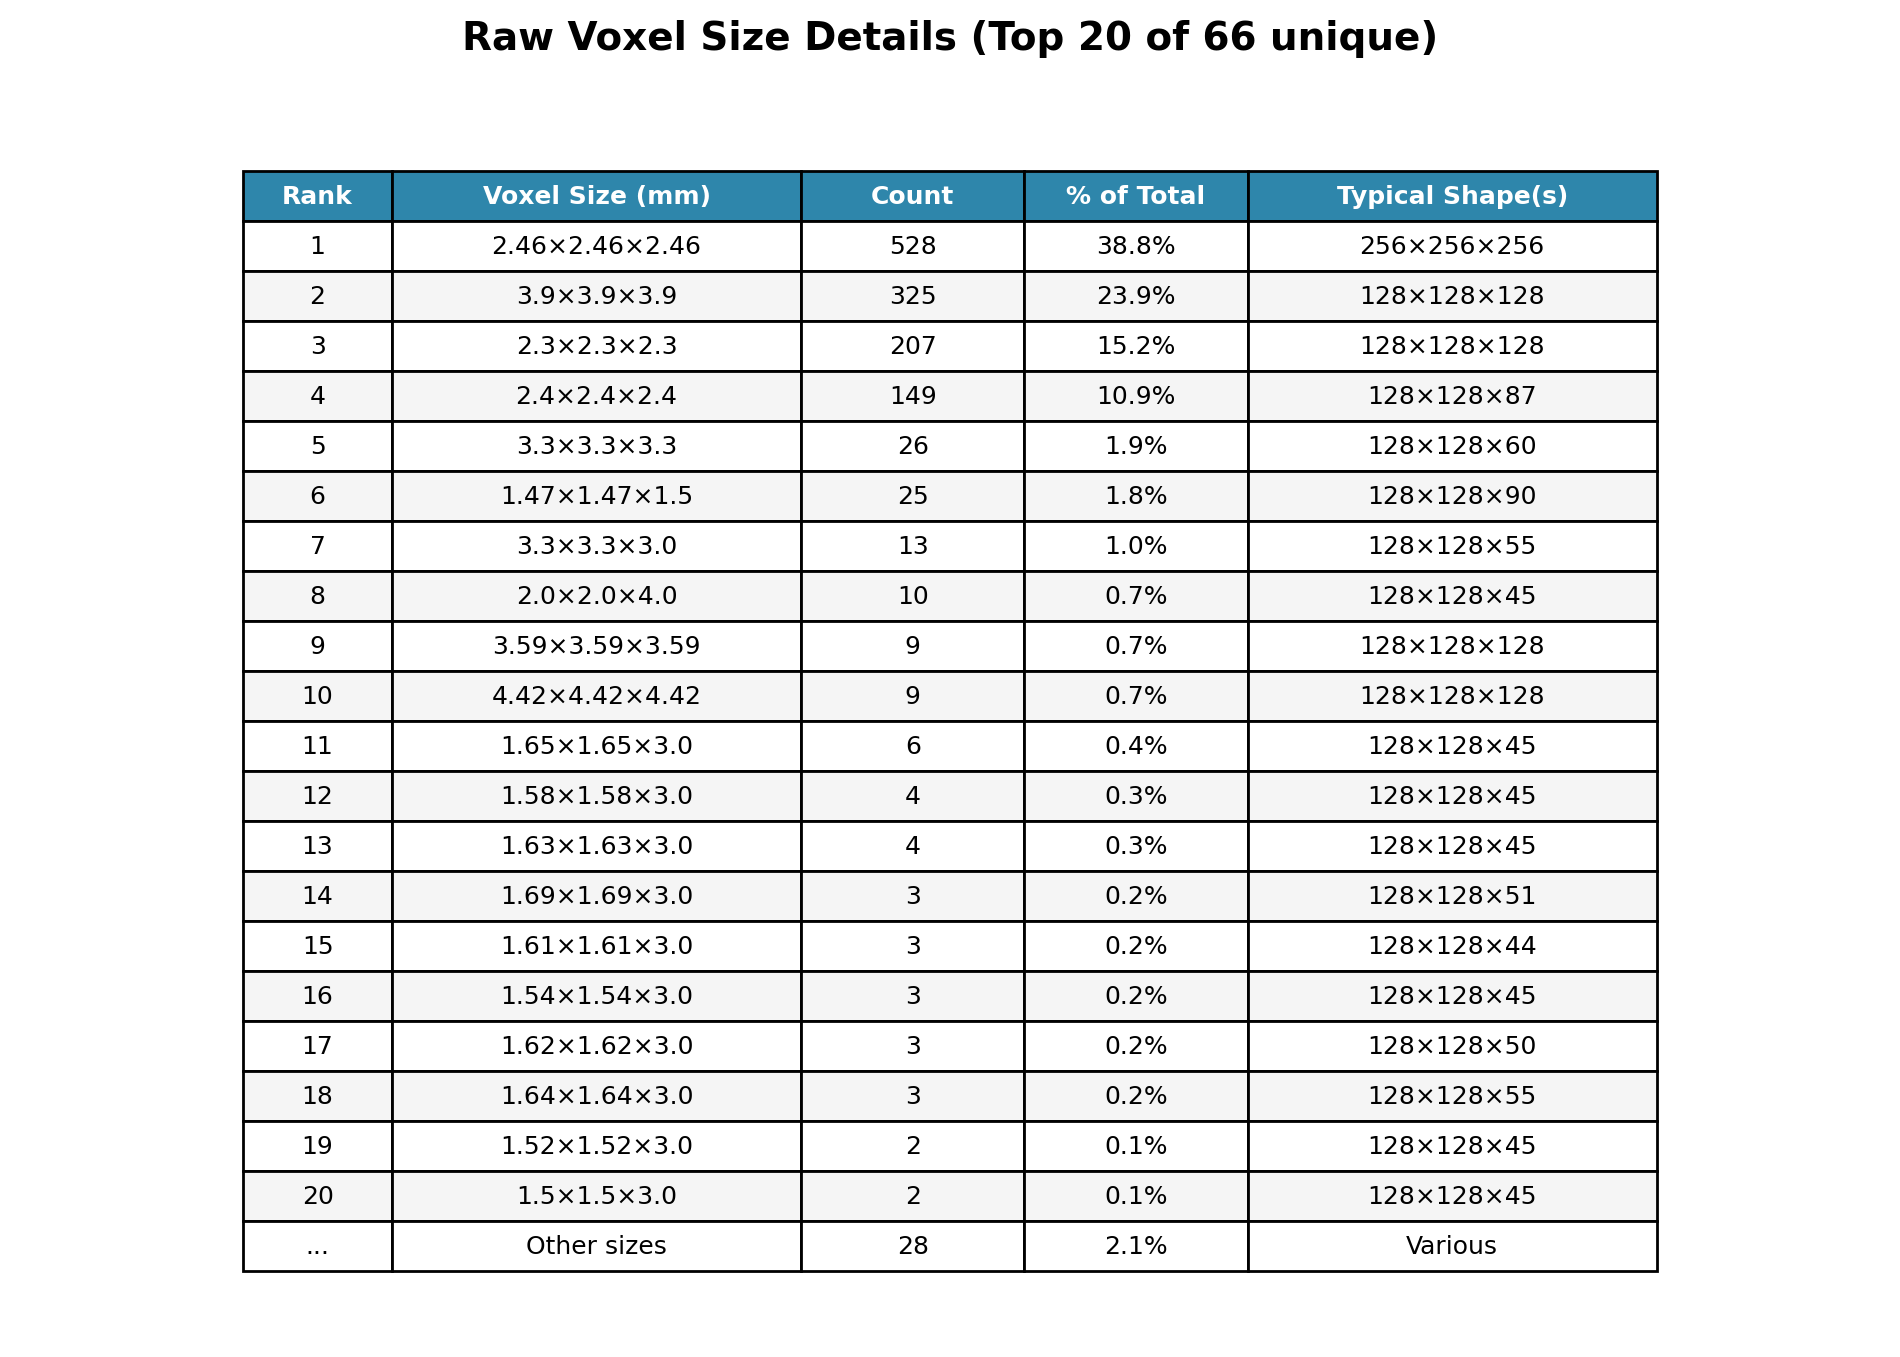
\includegraphics[width=0.8\linewidth]{figures/voxel_size_details.png}
    \caption{Detailed voxel size table (top 20 of 66 unique sizes). Shows count, percentage, and typical shape for each resolution.}
    \label{fig:voxel_details}
\end{figure}

\begin{figure}[htbp]
    \centering
    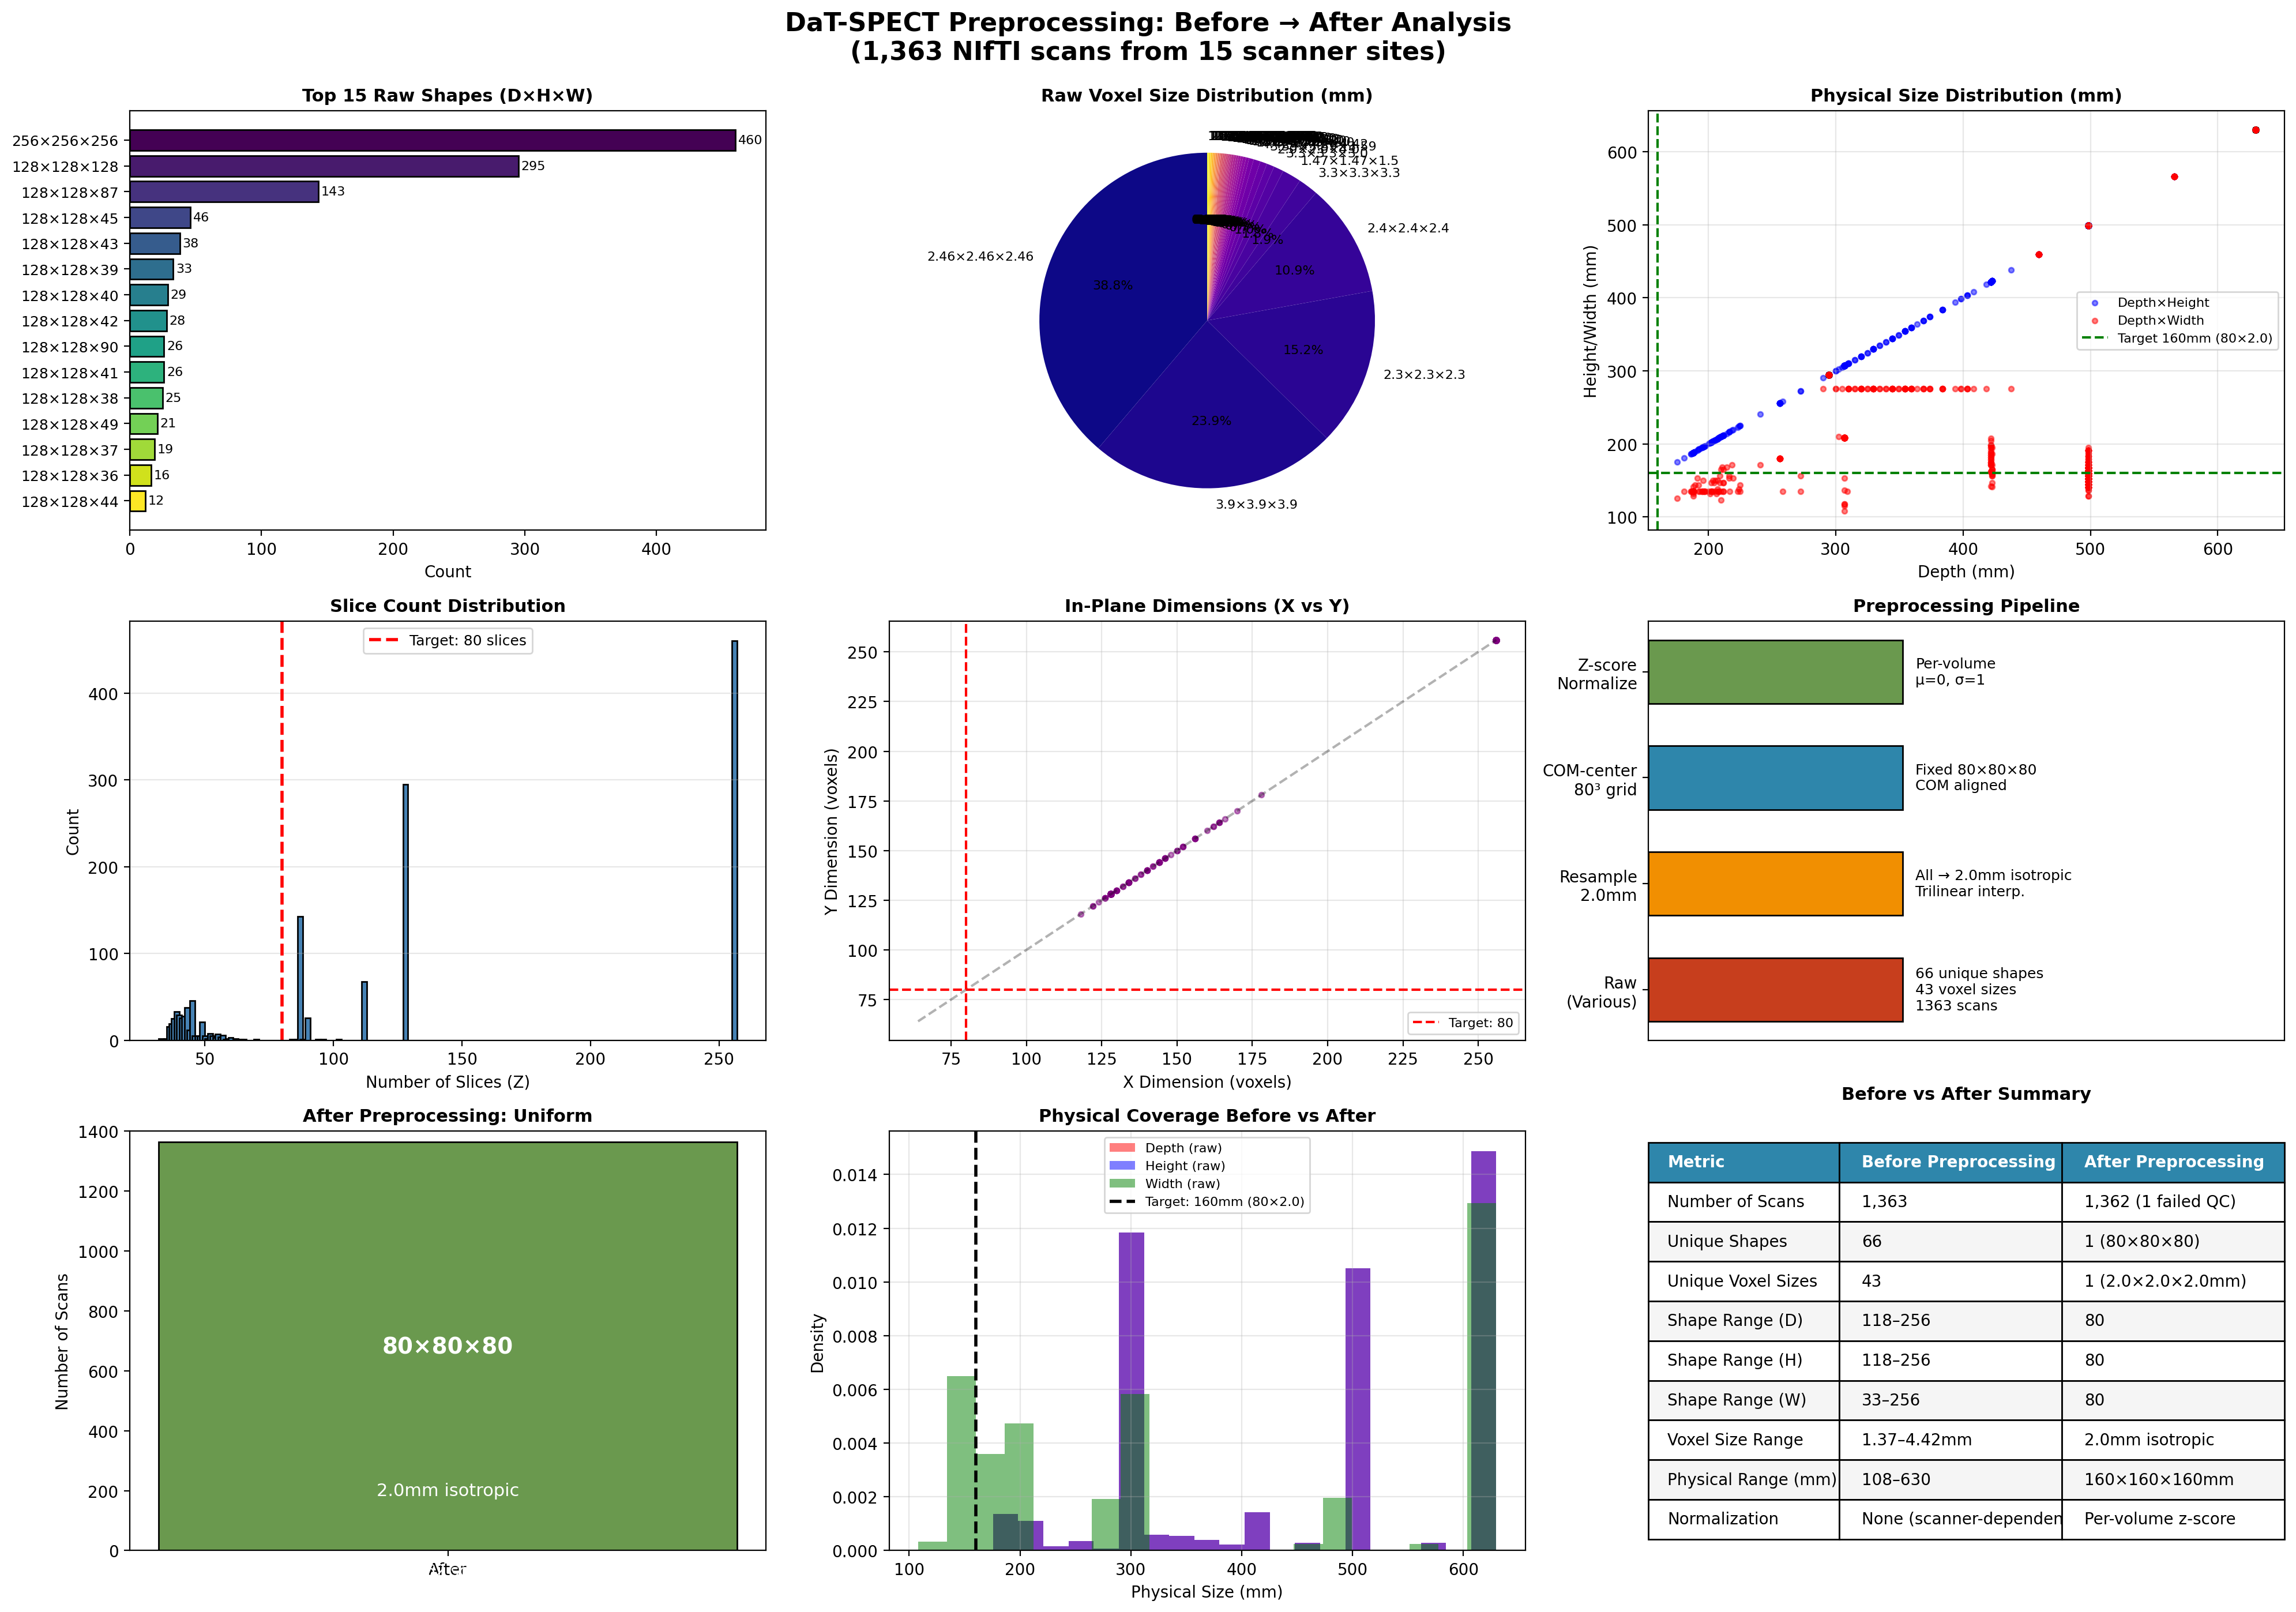
\includegraphics[width=0.8\linewidth]{figures/preprocessing_before_after.png}
    \caption{Complete before/after preprocessing pipeline with summary statistics.}
    \label{fig:preprocessing_full}
\end{figure}

\end{document}